% options:
% thesis=B bachelor's thesis
% thesis=M master's thesis
% czech thesis in Czech language
% english thesis in English language
% hidelinks remove colour boxes around hyperlinks

\documentclass[thesis=M,english]{FITthesis}[2019/12/23]

\usepackage[utf8]{inputenc} % LaTeX source encoded as UTF-8
% \usepackage[latin2]{inputenc} % LaTeX source encoded as ISO-8859-2
% \usepackage[cp1250]{inputenc} % LaTeX source encoded as Windows-1250

\usepackage{subfig} %subfigures
\usepackage{pdfpages}
\usepackage{csquotes}
\usepackage{amsmath} %advanced maths
\usepackage{amssymb} %additional math symbols
\usepackage{amsthm}
\usepackage{dirtree} %directory tree visualisation
\usepackage{todonotes}
\usepackage[outputdir=./tmp]{minted}
\usepackage{xcolor}

\newcommand{\tg}{\mathop{\mathrm{tg}}} %cesky tangens
\newcommand{\cotg}{\mathop{\mathrm{cotg}}} %cesky cotangens

% % list of acronyms
% \usepackage[acronym,nonumberlist,toc,numberedsection=autolabel]{glossaries}
% \iflanguage{czech}{\renewcommand*{\acronymname}{Seznam pou{\v z}it{\' y}ch zkratek}}{}
% \makeglossaries

% % % % % % % % % % % % % % % % % % % % % % % % % % % % % % 
% EDIT THIS
% % % % % % % % % % % % % % % % % % % % % % % % % % % % % % 

\nocite{*}

% \includeonly{
%  content/0-Introduction,
%  content/1-terminology,
%  content/2-framework-selection,
%  content/3-evaluation-criteria,
%  content/4-implementation
% }

\department{Department of Software Engineering}
\title{Object-relational mapping for database access in JavaScript}
\authorGN{Ladislav} %author's given name/names
\authorFN{Louka} %author's surname
\author{Ladislav Louka} %author's name without academic degrees
\authorWithDegrees{Bc. Ladislav Louka} %author's name with academic degrees
\supervisor{Ing. Jan Matoušek}
\acknowledgements{THANKS (remove entirely in case you do not with to thank anyone)}
\abstractEN{TODO Summarize the contents and contribution of your work in a few sentences in English language.}
\abstractCS{TODO}
\placeForDeclarationOfAuthenticity{Prague}
\keywordsCS{Replace with comma-separated list of keywords in Czech.}
\keywordsEN{Replace with comma-separated list of keywords in English.}
\declarationOfAuthenticityOption{1} %select as appropriate, according to the desired license (integer 1-6)
% \website{http://site.example/thesis} %optional thesis URL

\linespread{1.3}


\newtheorem{definition}{Definition}

\begin{document}

% \newacronym{CVUT}{{\v C}VUT}{{\v C}esk{\' e} vysok{\' e} u{\v c}en{\' i} technick{\' e} v Praze}
% \newacronym{FIT}{FIT}{Fakulta informa{\v c}n{\' i}ch technologi{\' i}}

\chapter{Introduction}

In the modern world, data have become an essential aspect of almost every field.
From e-commerce to healthcare, education to finance, data is everywhere and
plays a~critical role in decision-making processes. The advent of Web 2.0
\cite{Web2Oreilly}, which brought the concept of user-generated content, was
largely supported by connecting the Web to databases. Social media platforms,
for example, rely heavily on data to provide personalized recommendations,
targeted advertising, and other features that keep users engaged. Even
applications not working with the internet often need significant data storage
and, as a~result, the ability to manage and manipulate data has become a
critical skill for developers and organisations alike.

Relational databases such as SQL Server and PostgreSQL are by far the most
popular type of databases for data storage used in business-level applications.
These databases use the relational data model, which is based on tables with
rows and columns, to store and manipulate data.

Object-oriented programming languages and languages incorporating parts of the
paradigm, such as Java, Python, Ruby, and JavaScript, have gained
popularity \cite{stack-overflow-survey} due to their ability to create complex
software systems that can handle large amounts of data efficiently.
Object-oriented programming (OOP) is a~programming paradigm that represents
concepts as \enquote{objects} that have attributes (data) and behaviours
(methods). This makes it easier to write, maintain, and reuse code, which is
essential when working with large-scale software systems.

\newpage

Despite the popularity of object-oriented programming languages, there is often
a disparity between OOP languages and the relational data model used by many
databases. OOP languages are designed to work with objects, whereas relational
databases are designed to work with relations. This can make it challenging for
developers to work with databases using OOP languages. 

Object-Relational Mapping (ORM) has become a~popular solution for developers who
need to connect object-oriented programming languages with relational databases
\cite{Torres_Galante_Pimenta_Martins_2017}. ORM allows developers to work with
relational databases using object-oriented programming languages, eliminating
the need to write complex SQL queries. By abstracting away the details of the
underlying database, ORM allows developers to focus on the application logic and
reduces the amount of boilerplate code that needs to be written. This makes it
easier for developers to work with databases and reduces the potential for
errors. 

The thesis aims to conduct a~comprehensive analysis of the most popular ORM
packages and SQL query builders for Typescript. This analysis will provide an
objective measurement of their relative strengths and weaknesses in terms of
functionality, type support, performance, and package quality. Also included are
noncomparative examples of syntax and usage examples of the packages, to
illustrate strengths and weaknesses and to showcase the functionality of the
modules. By evaluating each package's performance in these key areas, the thesis
aims to provide a~comprehensive comparison that will be useful to developers who
are looking for the best ORM or SQL query builder package for their Typescript
project.

While there are existing comparisons, most of them are created from the point of
a biased actor, usually a~competitive or alternative solution developer
\cite{drizzleComparison} \cite{imdbBench}. This thesis aims to provide an
independent view.

% Before we start with the full comparison of ORMs that support TypeScript, we
% must first define what counts as an Object-Relational Mapping Package, what are
% SQL Query Builders, and other technologies and terms used further in this work.
% Then we explain how the packages further analysed were selected and by which
% criteria they are ranked and reviewed.

The thesis is organized into eight chapters that guide the reader
through comparing and benchmarking various frameworks.
\autoref{ch:preliminaries} sets the foundation by defining the terminology used
throughout the thesis and providing context for each term.
\autoref{ch:selection} focuses on determining the essential attributes for
a~framework to be considered for inclusion in the comparison.
\autoref{ch:RankingCriteria} then discusses the criteria used to compare and
rank the packages, from directly calculated comparisons to more qualitative
aspects like TypeScript support level and documentation quality. 

Chapters 4 through 8 delve into the practical aspects of the thesis, with
\autoref{ch:database} introducing the features of the Cat database, which serves
as the basis for testing the features and performance of the packages.
\autoref{ch:benchmarkDesign} outlines the design of the benchmark framework and
highlights the crucial features for implementation.
\autoref{ch:BenchmarkImplement} covers the actualization of this design into
a~functional benchmarking tool. \autoref{ch:Packages} presents an in-depth
analysis of individual packages, noting any problems or interesting findings
encountered during the implementation of testing tasks. Finally,
\autoref{ch:observations} synthesizes the results of the benchmarking process,
comparing and contextualizing the findings from both flexibility and performance
testing.
\chapter{Preliminaries}

In this chapter, we will establish a~solid foundation for the rest of the thesis
by introducing the key concepts and definitions used later in the work.

\section*{Object-Relational Mapping}
Object-relational mapping is a~way to access relational data in an
object-centred programming language \cite{agile-mapping-objects}. The primary
purpose is manipulating data without switching concepts from object-oriented
paradigms to the relational representation of data in which most databases
operate. The scope of this translation layer can (as shown later in this work)
vary. Different people define packages as ORMs while providing diverse levels of
functionality \cite{artima-abstractions}.

At its base level, ORM provides an intermediary layer between applications' OOP
model and database which is usually relational (but can be graph or document
focused). The layer allows the developer to work with objects in the code, while
the package translates it into a~relational structure when saved to the
database. These packages are often used on projects that are heavily connected
to a~database model, as ORMs are most beneficial when using a~database is
commonplace. When used only occasionally, it usually brings too expansive a
setup to translate into gains in code readability and maintenance costs compared
to executing premade SQL queries \cite{Torres_Galante_Pimenta_Martins_2017}.

In addition to the basic functionality of translating between different styles
of data representation, ORMs often include functionality such as connection
pooling, support for read-only data replications, caching, or database
migrations. When using such modules, developers can avoid writing boilerplate
code that is typically required.


\section*{SQL Query Builder}
SQL query builder is derived from its function to create SQL queries and OOP
pattern, which it implements, called \enquote{builder}. Object-oriented
programming design patterns are reusable solutions commonly encountered during
software development in OOP languages. These patterns propose interactions
between objects and their internal structure. There is no single authority on
how these patterns are defined, nor a~comprehensive list of these patterns, as
every author prioritises different patterns and functionalities
\cite{fowler-patterns-2003}.

The Builder pattern is one such pattern, providing API for the complex creation
process of objects. This pattern is one of the 23 defined in \enquote{Design
Patterns} by Erich Gamma, Richard Helm, Ralph Johnson, and John Vlissides
\cite{gamma-design-1995}, which has been highly influential in software
engineering. Its purpose is to separate the creation of an object from its
representation, allowing for the separation of parts that initially were parts
of one construction method into several.

SQL Query is made up of several clauses, which each serve distinct functions.
For example, the \texttt{SELECT} clause specifies which columns are to be
retrieved, and the \texttt{FROM} clause specifies which table or tables the
columns should be \cite{postgres-lexer}. Once the builder pattern is applied to
the SQL query, each of these clauses (or even smaller fragments) can be created
by calling the Builder's methods, creating a~programmatic way to create SQL
queries. The Builder also allows developers to abstract minor differences
between different SQL implementations.

As the ability to create queries based on multiple criteria is one of the basic
functionalities of ORMs, they are almost always built on top of a~query builder.
These can be available standalone or fully integrated into the ORM package.
Often, query builders are sufficient for the purposes of database access in most
applications, so they were included in the comparison. While they certainly lack
feature sets and, compared to ORMs, query builders usually require SQL
knowledge, they can be easier to set up and maintain while also being faster and
allowing fine-tuned adjustments to a~query.

\section*{PostgreSQL}
One of the most popular database engines today, PostgreSQL, is an open-source
object-relational database management system. Originally developed under the
name Postgres \cite{postres-about} (short for Post-Ingres) as a~new generation
after a~successful relational database called Ingress, it was first released
under this name in 1989. After several years of development at the University of
California at Berkeley, the name was changed to focus on SQL compliance. The
whole project moved to open-source, community-focused development in 1996.
Currently, the project is maintained by The PostgreSQL Global Development Group,
and releases and source code are provided under an open-source BSD-style licence
free of charge \cite{postgres-licence}.

PostgreSQL is, at the time of writing, one of the most popular SQL databases
available, owing its widespread adoption to its reliability and high scalability
while supporting most of the SQL standard and being fully ACID compliant
\cite{postgres-transaction}. ACID is an acronym for Atomicity, Consistency,
Isolation, and Durability, which are four fundamental tenets specifying
properties for reliability and consistency of transactions.

Some of the features that often make PostgreSQL stand out amongst other RDBMS
are its support for many different and advanced data types
\cite{postgres-datatypes} out of the box, such as the ability to natively store
JSON objects and arrays, XML data or geometric types. With extensibility being a
significant focus, a~lot of functionality can be installed or optionally
enabled, further improving the reach and applicability.

There are extensive implementations of the API for many programming languages,
including C \cite{libpq}, Python \cite{psycopg2}, Java \cite{pgJDBC}, and
JavaScript \cite{node-postgres}. PostgreSQL also offers extensive documentation
of both its API and internal functionality, which supports its growth and
popularity.

\section*{Lazy loading}
Lazy loading is a~technique for optimizing data retrieval to increase
application performance \cite[p.~200]{fowler-patterns-2003}. It is a~strategy consisting of
only loading data when it is needed rather than all at once, therefore reducing
the initial load in exchange for the need to do additional loading later. Lazy
loading is usually achieved by breaking down larger datasets into smaller ones
and loading each one only when necessary. Such practice is commonplace in web
development, as asset sizes (such as images or JavaScript) have only grown in
the evolution of the web.

Some of the most common implementations of Lazy Loading come in the way of only
loading low-quality images unless the user is focused on them or splitting code
into multiple files, which are fetched when necessary, providing quick first
page-load time at the cost of adding additional requests
\cite{webPerformanceMDN}.

When talking about ORMs and database access, lazy loading usually takes place as
replacing data retrieval from an object with a~call to retrieve the data from
the database. In other words, the data of the database object does not need to
be loaded when the object representation or its part is created in the program.

\section*{Eager loading}
Eager loading is the programming practice of loading all the required data at
once, optimizing the number of requests that must be made to retrieve everything
\cite{sequelize-eager-loading}. This is done with the expectation that one
expensive request will minimize the amount of additional data that would need to
be sent between the two parties. This can lead to faster load times and improved
application performance.

It is usually achieved by sending a~singular request and caching the data in
memory, even though it might only be needed later. There are obvious downsides
to this, such as higher memory usage or often loading more data than is
necessary. The concept of eager loading is antithetical to the lazy loading
approach, and that is on purpose. Each approach prefers a~different focus, and
thus each is fit for different usage; lazy loading is practical when a~first
look or first results matter the most, and eager loading is when the focus is on
one large result, which would be slowed down by too many small requests, which
would need to be made for the total result.

In the context of object-relational mapping frameworks, we are most likely to
encounter eager loading when fetching related entities. This way, when there is
an expectation for data about the currently approached entity, the ORM can
optimize the query so that the data are already loaded in memory when it is
requested later.


\section*{Circular dependence}
A common problem in software development, circular dependency occurs when two or
more parts of code depend on each other, making it impossible to resolve their
dependence onto a~dependency graph. Such a~graph must conform to limits set out
for tree graphs and, therefore, cannot contain a~loop. Due to the way how
modules are loaded in Node.js \cite{commonjsModulesNode}, such a~problem would
lead to a~deadlock and is therefore resolved by trying to run the modules in a
specific order. However, such an approach is only sometimes feasible, so other
solutions must be used. The issue of circular dependency is also present in the
compilation because, while TypeScript does allow asynchronous references of
types between files using \texttt{import type} term \cite{typescript-modules},
if we need to import not only the type but also the value, TypeScript will not
be able to resolve the type, and the compilation will fail. There are many
solutions to this problem, the most common being dependency injection or lazy
loading.

In ORMs and database representation in OOP languages, this problem is generally
connected to the bidirectional nature of relations, as its explicit
representation will inevitably create circular dependency
\cite{melton-empirical-2007}. Therefore, for most schema definitions, there
needs to be a~functionality built in that allows users to define bidirectional
relations without sacrificing type safety or encountering a~deadlock with
importing modules. 


\section*{Database transaction}
Transaction isolation is a~concept used in database management to represent a
unit of work. The transaction is typically a~series of one or more database
operations that are supposed to be completed on the all-or-nothing principle. In
addition to performing database queries atomically, the transaction also needs
to provide additional functionality, such as coordination of reads and handling
operations in a~reliable and recoverable manner. 

As database transactions are the base for the basic functionalities of modern
RDBMS \cite{haerder-principles-1983}, their handling is essential when
considering the ORM framework. Often an operation can only be performed when the
previous one succeeded or has to be made strictly in order without another
operation having access to the data in between \cite{postgres-transaction}. This
can be achieved only through the database transaction, and support for them is
necessary for many use cases.


\section*{Database connection pool}
A database connection pool is a~component that collects and manages several
database connections and allocates them to individual requests to the database.
It works by creating either a~fixed number of connections at the beginning or
scaling up the number of connections based on usage. In this way, querying the
database does not have to wait for the connection to be established, and the
request can be routed through the database connection pool to the currently
unused connection \cite{gupta-improving-2017}. Additionally, due to having
multiple connections, multithreaded and asynchronous applications can coordinate
connections to the database. Single connection applications can be stalled while
waiting for a~single otherwise non-blocking request, while others could be
served by the database. Such connections must be coordinated with transaction
management, as the transaction is inherently connected with the connection that
spawned it. 


\section*{Read replica}
A read replica is a~special kind of database instance, a~read-only instance of
the database presenting additional query points for the applications accessing
the database without having to resolve consistency between instances. Some
databases support multiple fully functional instances, however concurrent writes
to alternative machines could produce an inconsistent state in the database.
With a~read-only replica, consistency is not threatened; the only negative is
the possibility that the connections will receive a~state that is delayed when
the replica is not synced to the latest consistent state of the primary instance
\cite{postgres-availability}.

Creation and usage of read replicas can significantly speed up application
performance as database queries are no longer constrained by single hardware
instance, which usually bottlenecks query speed. Duplicating the data over two
instances can double disk read speeds; if different physical devices are used,
slow scans over data can run independently and finish faster.


\section*{JavaScript}
A high-level dynamically typed programming language developed in the mid-1990s
at Netscape Communications Corporation to add dynamic content to web pages.
Initially called Mocha, it was later renamed multiple times to finally settle on
JavaScript to use the (at the time very high) popularity of Java
\cite{auth0JavascriptHistory}.

Before JavaScript, websites were almost always purely static documents that were
displayed in web browsers (such as Netscape at the time or Google Chrome or
Firefox currently). The logic for any web application had to be handled purely
on the server side. With the introduction of JavaScript, web pages were able to
be more interactive and dynamic. While initially designed to be used when
writing HTML documents and executed by web browsers, it outgrew its client-side
roots and conquered large parts of the server-side development and even mobile
app and desktop application environments. The advantage of JavaScript is that it
can be a~completely full-stack language which provides exact parity of logic
between client and server and allows for significant code portability.

Until the last few years, JavaScript had an exclusive reign over interactive web
content, which made it one of the most used programming languages in the world
\cite{stack-overflow-survey}. With multiple deficiencies known and unfixable
without massive problems with incompatibility, multiple additions which build
atop JavaScript and even whole languages which compile into JavaScript were
developed. Some complied languages are, for example, CoffeeScript
\cite{coffeescript-homepage}, Dart \cite{dart-homepage} or TypeScript
\cite{typescript-homepage}. These languages exist to provide additional features
and functionality that are not easily or at all possible in pure JavaScript.


\section*{ECMAScript}
Soon after the introduction of JavaScript, it became apparent that establishing
standards would be a~necessary step for compatibility between implementations in
different web browsers. Following this consensus, ECMA (originally an acronym
for European Computer Manufacturers until 1994 \cite{ecma-mission})
International standards association meeting was held, and the first edition of
the document specifying the new standard specification was adopted in June 1997.

The specification, coded under the name ECMA-262 \cite{ecma-262}, is a
comprehensive document that has gone over several versions over the years and
specifies the syntax, semantics, and behaviour of the language. There is also an
extensive description of data types, operators, flow control structures,
built-in objects, and API.

ECMAScript is currently used primarily for client-side scripting, with primary
implementations being those used in web browsers, such as SpiderMonkey (Firefox)
\cite{spidermonkey-documentation}, V8 (Google Chrome, Opera) \cite{v8-homepage}
and JavaScriptCore (Safari) \cite{javascript-core}. Increasingly with new
revisions of the standard, even server-side applications and services have
started migrating to ECMAScript from other standards (primarily CommonJS), but
many constructs are not directly compatible or translatable.


\section*{CommonJS}
One of the alternative specifications which reflected missing functionality in
ECMAScript for server use is CommonJS. Created to establish conventions on
modularization for JavaScript outside the web browser, it has also standardized
several APIs and internal features \cite{commonjs-spec}. 

Started in 2009 by an engineer at Mozilla, the project was initially called
ServerJS, with its flagship feature being the synchronous loading of modules.
This means that once a~module is imported, its exported components are
immediately available to be used \cite{commonjs-introduction}. This simplifies
working with modules and was necessary for the expansion of JS code into
server-side development and is used widely today. 

Since its conception, gripes with the ECMAScript specifications were largely
fixed with further iterations, making it also usable in server-side development.
Popular packages, including those exclusively used in server development, have
migrated their codebase to ECMAScript.


\section*{TypeScript}
A statically typed language built on top of the JavaScript foundation,
TypeScript was developed by Microsoft Corporation with the focus on allowing
developers to catch errors at compile time before the problem is encountered
during runtime, which usually requires extensive testing. TypeScript code is
written in enhanced syntax and then compiled into regular JavaScript, with
several standards supported, including CommonJS and ECMAScript
\cite{typescript-modules}.

TypeScript was designed to address several shortcomings that have been present
in the ecosystem for a~lost time, especially when creating large-scale
applications. JavaScript applications are very flexible with their dynamic and
loosely typed nature and prototype usage, but with flexibility comes a~large
surface area for errors and mistakes. 

Today, TypeScript is widely used for web development and JavaScript server-side
development. Most popular frameworks provide at least partial support for
TypeScript, and some (such as Angular and React) have even switched to it as the
recommended language. TypeScript has support in many JavaScript-integrated
development environments, such as Microsoft's Visual Studio Code
\cite{typescript-vscode} or JetBrains WebStorm \cite{typescript-webstorm}. With
solid typing comes the ability for more substantial and consistent code
completion, guaranteed automated refactoring, and error checking.

Other projects have tried to fix the same issues as TypeScript fixes. For
example, Dart \cite{dart-homepage}, which is developed by Google, works in the
same way, although it abstracts further from the traditional JavaScript syntax.
It is also compiled into standard ECMAScript syntax. However, it never gained
the same traction, and its focus was changed from alternative to JavaScript to
the primary language for development in the multi-platform framework Flutter.


\section*{Node.js}
Node.js is an open-source, cross-platform JavaScript based on the V8 engine,
which was originally developed by Google for Google Chrome. It is designed to
allow for server-side usage of JavaScript, with focus on network applications
\cite{node-about}. Released by Ryan Dahl in 2009 \cite{ryan-node}, it has since
become standard for server-side JavaScript development, especially web
applications. The framework has gained popularity thanks to its alternative
execution model, which separates it from traditional server-side languages.
Instead of spawning different threads or workers for connections, it works with
a non-blocking asynchronous I/O model, where many concurrent connections can be
handled with only a~small overhead \cite{orsini_2013}.

This is achieved through asynchronous programming, where multiple tasks can be
executed concurrently without blocking the main execution. Node.js supports
asynchronous programming through the concepts of callbacks and promises.
Callbacks are functions passed as arguments that are executed in finished or
failed states, ensuring that logic can be applied sequentially after the
asynchronous operation is finished. Promises provide a~more structured and
object-focused way to handle asynchronous operations and have become the
preferred way. a~promise is a~representation of value which might not be
available yet, containing a~status variable and reference for the result once
achieved, allowing for code execution while the operation status is updated in
the background. When the value of the promise is necessary, the promise can be
checked or awaited by using the async/await constructs
\cite{PromiseJavaScriptMDN_2023}.

While Node.js is currently the most dominant, there are other alternatives
available with their own approaches and focuses. The most popular one is Deno,
also developed by Ryan Dahl, with the intention to address some of the security
and design issues of Node.js. Deno, for example, contains extensive tools and
utilities within its standard library or uses better sandboxing between modules
as supported by V8, the engine on which both it and Node.js run \cite{Deno}.

\section*{npm}
One of the key benefits of the Node.js ecosystem is the large number of
third-party packages that can be incorporated into projects. For example, many
popular web frameworks, such as Koa or Express.js, are built for Node. 

Originally an acronym for Node Package Manager \cite{npm-old-readme}, the
three-letter name has been retroactively stripped of such meaning
\cite{npm-usage}. The first release was published in 2010, and it has since
become the default Node.js package manager. Npm consists of a~command line
client, which is also called npm, and an online database of packages called the
npm registry, which is hosted at \url{www.npmjs.com}. 

Although npm is the default package manager, alternatives that were created with
different focuses and compromises exist, for example, yarn \cite{Yarn}, although
they usually don't provide their own registry.

\section*{JSON}
JavaScript object notation (JSON) is a~lightweight data-interchange format that
is widely used in web development. Introduced as an alternative to the complex
XML format that was previously used, it is based on a~subset of JavaScript
representation of values. It consists of key-value pairs in objects, arrays, and
primitive types. One of the main benefits is its simplicity and readability for
humans, which makes it useful for places where data could need to be interpreted
by both humans and machines.

JSON has been standardised in the ECMA-404 \cite{ECMA-404} document by Ecma
International. The document specifies syntax and semantics, ensuring its
reliability, consistency, and portability throughout systems and applications.

\section*{Unit of Work}
Unit of Work is a~software design pattern used most commonly in ORMs and similar
frameworks to manage persistence and consistency between application and
database state. The pattern is used to group all database operations relating to
a single transaction or process and only execute the final state, ensuring they
can be performed atomically without requiring lengthy and expensive locking of
database rows or tables or risking deadlocks through database transactions
\cite[p.~184]{fowler-patterns-2003}.

The main idea is to track changes across the object in memory, and instead of
committing every change into the database, only the last state change is
executed. This can be applied not only across one object instance but also
across whole swathes of objects. While atomicity is undoubtedly necessary on
many occasions, and unit of work on the ORM side can significantly reduce the
number of requests to the database, it can also lead to inconsistency when
multiple applications access the database and data which are currently loaded in
memory on one machine are modified by a~different one.

\section*{Active record}

\begin{figure}[t]
    \caption{Active pattern class diagram, recreated from Patterns of Enterprise Architecture}
    \centering
    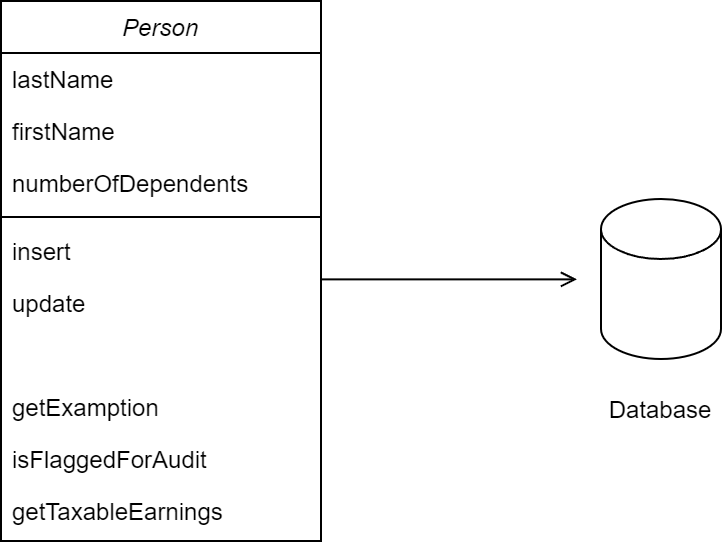
\includegraphics[width=0.6\textwidth]{ActiveRecord}
\end{figure}

The Active Record pattern is a~design pattern defined by Martin Fowler in his
book "Patterns of Enterprise Application Architecture"
\cite[p. 160]{fowler-patterns-2003} and is commonly used to represent database
records in an application.

The goal of the pattern is to encapsulate logic for interacting with the
database table into a~single object. Each instance of the object represents a
single record, and modifications made on it are then usually flushed with a
method call into the database. The base class also provides static methods for
CRUD (create, read, update, delete) operations and possibly additional business
logic.  

The main benefit of the Active Record pattern is a~simple and intuitive
interface for objects and tables. Modifications of the object can be made right
on the data in languages, which allow setters and getters on attributes, and
static methods provide a~simple gateway to work with the table. 

Limitations of the pattern come in the tight coupling between the application
and database logic, as the object instance is inherently tied to the database
representation. This makes it harder to test the implementation and often
requires additional abstraction or mocking. Additionally, the pattern does not
easily allow for the management of relations, so a~database schema with complex
relations might not be able to represent the data easily. 

\section*{Data mapper}

\begin{figure}[t]
    \caption{Data Mapper class diagram, recreated from Patterns of Enterprise Architecture}
    \centering
    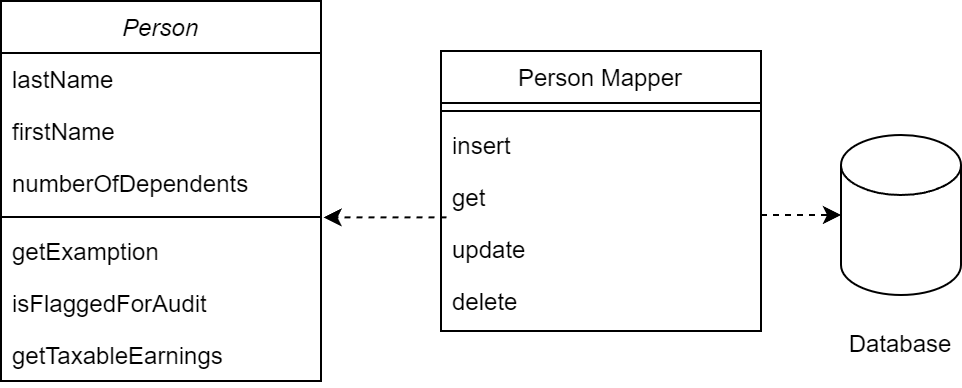
\includegraphics[width=0.8\textwidth]{DataMapper}
\end{figure}

The Data Mapper pattern, as described by Martin Fowler in his seminal work on
enterprise application architectures, provides a~clear separation between domain
models and their underlying data storage. This approach enables developers to
create complex and expressive domain models without being constrained by the
relational database schema or various storage options. By decoupling in-memory
representations from the data storage mechanisms, the Data Mapper pattern
promotes a~clean separation of concerns and enhanced flexibility in application
design \cite[p. 165]{fowler-patterns-2003}.

Distinguished from the Active Record pattern, the Data Mapper pattern ensures
that business logic and data access responsibilities remain separate. In this
approach, a~single entity represents the table or collection, while distinct
entities represent individual records. The Data Mapper serves as a~data access
layer that performs operations on the data storage representation without
creating any direct bindings between in-memory objects and the database. This
responsibility is solely managed by the Data Mapper, which takes care of any
objects that utilize it.

By limiting the responsibilities class must service and ensure that it is not
accountable for multiple unrelated tasks, the single responsibility principle
aims to create more straightforward and more maintainable classes. Consequently,
the Data Mapper pattern contributes to a~more robust and modular software
architecture that is easier to develop, maintain, and extend.

However, the Data Mapper pattern has drawbacks. One notable downside is the
increased complexity introduced by the additional layer of abstraction. This
added complexity could lead to a~steeper learning curve for developers
unfamiliar with the pattern, as well as the potential for increased development
time. Moreover, the mapping process between domain objects and the persistence
layer may introduce performance overhead, which can be a~concern for
applications with stringent performance requirements.

\setsecnumdepth{part}
\chapter{Framework selection}

Selecting the optimal framework for any project can be difficult with many parameters and options, and quite often, there are better options than the most popular. The JavaScript ecosystem is rich in choice, as throughout the years, many developers and companies have aimed to create packages in their image. Mainly due to this plethora of choices, there is a need for an overview, which would present advantages and disadvantages. However, only some frameworks can be reviewed; therefore, at least essential criteria need to be established. \par
The selected packages were selected for their support of TypeScript, with varying levels of compatibility, which will be shown in further detail later. Additional criteria considered were popularity and support as separate factors, leading to the inclusion of widely-used packages with currently limited support and development and lesser-known packages with solid support. \par
\section{Typescript support}
The primary selection criterion for the packages was TypeScript compatibility. Each package had to have at least a basic functionality working and typed, requiring only reasonable effort to integrate. The degree of support varies among the packages, and their level was also measured in comparison, but the base level was necessary to be considered.\par
The functionality considered essential is not easy to define either, but as the level of type support varied, the minimum settled on was package and connection setup and simple querying. The package had to have connection options typed, at least for primary usage, as listing all options for all connections is not necessary for most uses. Querying and updating database records is the most common activity for which ORMs and connection builders will be used, so the types they provide are some of the most useful. The result of a simple non-joined query on one table should be able to return exact and correct types, and an update of the record should also at least suggest the attributes which can be changed.\par
\section{Popularity and Support}
Popularity was inherently a factor in the selection of packages; if the package was known more, its likelihood of being found was smaller. We researched popularity in several ways; the primary source was searching by name and keyword ORM on the npm repository. Secondary sources were articles on ORM and database access in Node.js. The npm repository provides statistics about the packages listed on it, the most prominent being weekly downloads. The statistic is good for basic orientation but is not a great indicator of the exact number of users, as users can download the package multiple times, most packages are cached by third parties, which automatically download a version when it is released and many more ways, which skew the number. Additional input for popularity was the number of issues and stars the project currently holds on GitHub.\par
Support is a secondary attribute that is highly linked to popularity. Although all packages reviewed are open-source, only maintainers can merge code into the main branch or release versions onto the registry. If they are no longer active, the project effectively stops. While they can be released under a new name if the licence permits such a thing, no packages missing implementation into the benchmark have forks that would relieve the issues encountered. High-quality support is crucial for addressing issues, incorporating new features and compatibility with changes in underlying technologies.\par
\section{Implementation criteria}
Although some packages were initially selected for comparison, as previously mentioned, problems that needed to be more severe were encountered during their implementation into the included benchmarks. They will still be introduced, and the issues explained; however, they will only be included in comparisons within the basic summary.
\chapter{Ranking and Grading of the Frameworks}

This chapter outlines and explains the criteria for evaluating ORM and SQL query
builder packages chosen for the comparison. These criteria will be the core
points which will be considered, but other specific notes will be made about
each package. The main criteria were the level of TypeScript support, range of
compatible database management systems, popularity, support, documentation
quality, dependency count, and performance in different scenarios.

\section{Quantifiable Criteria}

The main section of the evaluation criteria focuses on technical aspects of the
frameworks, specifically their usage of TypeScript, support for different
databases, and difficulty composing queries. As these qualities are
quantifiable, they were given the highest priority in comparing the packages.

\subsection{TypeScript Support}

The quality and extent of TypeScript support vary among the packages, with some
offering better integration and type safety without the need for casts. In
contrast, others only provide basic typing or require result type definitions to
be written into each request, which amounts to the same behaviour as if the
result was cast. Such functionality often comes when the package initially
written for JavaScript is not rewritten in TypeScript but is only provided with
a \texttt{types} file, which specifies call signatures, but cannot provide other
assurances.

\subsection{Database Compatibility}

Wide database compatibility is necessary when working with a~large project that
may encompass many services or when choosing a~toolchain for a~team working with
dynamic technology stack, as the one database may not satisfy all the needs the
team might have, and building experience with multiple frameworks could be
considered unnecessary spending. Providing a~unified API over multiple databases
can be one of the benefits of query builders or object-relational mapping
frameworks.

\subsection{Flexibility and Performance}

Flexibility and performance are crucial in a~database access framework. Suppose
the package would restrict the ability to access the data, requiring roundabout
ways to deal with basic operations. In that case, there are better ways to
simplify development, just as if the framework creates excessively suboptimal
queries or adds excessive overhead. One of the requirements for a~comprehensive
ORM framework is the ability to support many use cases and represent and work
with many different data models. If ORM doesn't support possible use cases or
cannot represent commonly used database design patterns, it is lacking in some
ways compared to one that does.

Performance is often secondary when choosing an ORM framework, as quite often,
even frameworks adding significant overhead and creating suboptimal queries are
usually not noticeably slowing down the application. As the application grows,
the performance can become significantly more critical, and the resources needed
can be more expensive to scale. a~high-performing package can support this
growth by maintaining efficacy under load and effectively using its available
resources.

Performance was measured in multiple ways; the first metric was the execution
time of a~single query to measure the latency added by using the framework,
compared to using other frameworks or plain database drivers. Benchmarking this
way provides information about the amount of overhead the framework requires to
function, and if the connection pool is well initialized, connections are
assigned optimally, and data are correctly retrieved. The second benchmark run
repeats the test multiple times to eliminate any inconsistency that could occur
in a~single run.

\subsection{ECMAScript and CommonJS compatibility}
There are two different primary standards for JavaScript syntax, ECMAScript and
CommonJS. They primarily differ in how the inclusion of modules is written and
the mechanism of the module import. While CommonJS was dominant in the server
backend space for a~long time, however, ECMAScript modules are becoming
significantly more popular, with support added in Node.js, TypeScript and many
popular packages.

Combining packages from both ecosystems can still lead to problems. The best way
to support all possible combinations is to provide both types of dependency
declarations.

\subsection{Licence}
As developers consider integrating packages into their projects, it is crucial
to consider and understand the significance of licences governing their use.
Open-source software is often regarded as a~valuable resource, offering a~large
amount of reusable code and often the best solution. However, it is essential to
understand that open-source does not necessarily equate to unregulated use.
Licences still dictate the terms under which the package and its code can be
employed, modified and redistributed. Therefore, developers must examine the
licences of potential packages to ensure their intended use aligns with the
terms granted.

The most permissive licences allow for usage, modification and redistribution
with at most a~requirement to credit the original author/authors and don't
require the licensee to maintain the same licence in derivative works. Examples
of such permissive licences are \textit{MIT License} \cite{MITLicense} or
\textit{Apache License 2.0} \cite{ApacheLicense2}. These are generally preferable
for projects that demand flexibility in their use of the software.

While still free, the opposite side to the permissive licences are copyleft
licences, which impose more stringent requirements on the usage, especially
modifications and redistributions of the software. The primary example of such a
licence is \textit{GNU General Public License} \cite{GNUGPL}, which requires
derived works to be distributed under the same licence.

Since copyleft or other provisions might limit the usability of libraries such
as ORMs for many projects, it is necessary to include the licence as a~grading
criterion.

\section{Package Properties Criteria}

However, technical criteria are only some that should be considered when
selecting a~framework. Many of these factors are interconnected; often, success
in one is either caused by or preceded by doing well in others. For example,
while the popularity of the package can show the reliability and usability of
the package, it also often results in more issues being reported, and more
users are more likely to create community resources supplying or improving
official documentation.

\subsection{Popularity}

Popularity measures usage, as indicated by package downloads, the number of
issues, and the number of users on GitHub who have shown interest in the
repository. While all imperfect measures for absolute popularity, they help
compare popularity between packages by their relative difference. In the case
that the package usage requires multiple dependencies to be installed, for
example command line interface for development and runtime dependency, the
highest number is listed.

\subsection{Support}

The number of resolved and still open issues can be used to show popularity and
support of the project. With such a~metric, support can be measured; however,
more important than that are the patterns of behaviour which maintainers have
shown previously. If the release schedule is predictable, bugs and security
issues are fixed quickly, hesitant adopters can be assured that this pattern
will continue, and the framework is a~safe investment. On the contrary, a
project which is officially or probably no longer supported can be assumed to be
a wrong choice, as it cannot react to newly found errors and problems with
dependencies and might be unusable due to changes with TypeScript or Node.js
runtime.

\subsection{Dependencies}

As dependencies require maintenance due to their changes and vulnerable
versions, their amount should also be manageable. Otherwise, it might increase
the maintenance cost for the package and application size. Even though data
storage is less critical than previously, having a~more storage-conscious
package is still beneficial.

\subsection{Documentation Quality}

Documentation quality is critical for new adoption and onboarding for working
with the framework. It also cannot be measured with reasonable objectivity.
Perceived quality depends on language understanding and users’ previous
experience with the programming language and similar frameworks. Evaluation of
documentation will therefore summarize clarity, extensiveness and whether
features such as JSdoc annotations \cite{Typescript-jsdoc} which can be parsed
by IDEs are used to contain or link to the documentation.


The following chapters aim to provide a~comprehensive and in-depth analysis of
packages compared by evaluating each package by these comprehensive criteria
with additional added when.

\chapter{Benchmark database schema design}\label{ch:database}

\section{Introduction}
This chapter describes the database used for performance testing of the ORM and
query builder packages. The database is designed around imaginary data
collection about cats, their home domiciles and toys found within these houses,
and the toys' manufacturers. The database comprises six main entities -
\texttt{cat}, \texttt{cat colours}, colour \texttt{hex codes}, \texttt{houses},
\texttt{toys} and \texttt{toy producers}.

\section{Cat Entity}
The \texttt{cat} entity instances represent individual cats which we want to
monitor. Each has a unique identifier, name and date of birth, all of which are
nullable except for the identifier. This entity aims to represent the basic
database table and to verify the correct handling of the data type from
Postgres, as JavaScript Date time represents a moment, including time. In
contrast, the database entry would only contain the date. Additionally, the
\texttt{cat} entity uses big integer data type, and handling numbers beyond the
standard range allocated in JavaScript is tested. The \texttt{cat colour} and
\texttt{colour hex code} are two entities that represent the cat colour by its
name and by its hex code. The entities are intentionally split in this way to
use identifying relation - the primary key of the hex colour entity is also a
foreign key referencing the id of the cat colour entity.

\section{House and Toy Entities}
The \texttt{house} entity represents domiciles where the cats spend their time
at their behest. The relation must also account for ambitious cats using several
houses as their homes. The main aim is to test the difficulty of implementing
and using simple many-to-many relations. The only attribute that provides new
data type or behaviour is the simple \verb|has_dog| attribute, specified as a
Boolean. It is one of several attributes that test the frameworks' ability to
correctly type and convert the data recovered from the database.

The houses can be equipped with many toys for the cats to use. The relation
between houses and toys is modelled through a decomposition table which contains
attributes representing the number of the same toy in the house. While the
primary keys are the identifiers of the house and toy, the decomposition with
the amount, rather than several records with an additional identifier, is
designed to test the ability to insert a record if it does not exist or update
the value referencing its previous state. If more toys are purchased, the owner
of the house does not suddenly throw out all toys they already had; they will
add them to their current pile. This operation is often called \textit{upsert} -
a combination of update and insert, and some database engines, such as
CockroachDB, implement it explicitly under this name. PostgreSQL achieves it
using the \texttt{ON CONFLICT} statement in \texttt{INSERT} query. It also tests
the handling of composite primary keys, a standard paradigm in many databases.

\section{Toy Entity}
The \texttt{toy} entity purpose in testing is in numeric data type used in
\texttt{price} attribute and usage of additional column attributes such as
\texttt{CHECK} constraints or \texttt{DEFAULT} values in the column. Column
\texttt{naughty} is focused on commonly problematic strings in software
development, such as special Unicode characters, emojis and other issues that
could come up in handling data from the database, especially if the encoding is
not correctly handled. Toys producers host the JSON columns to test if it is
possible to use advanced JSON traversal and query operators provided in
PostgreSQL (and their equivalents in other database management systems).

\chapter{Benchmark Framework Design}

The benchmarking process was designed to compare the performance of various ORM
and SQL query builder packages. As such, it was important to ensure that the
benchmarking framework was developed in the same environment as the packages
themselves. To achieve this, the framework was implemented in TypeScript, the
same language used by the packages being tested.

The benchmarking framework had to be designed to accommodate errors that could
occur during development and testing of the packages. Additionally, it has to
support testing of multiple database schemas and allow for results to be
exported in a~variety of formats for further analysis. The resulting
benchmarking framework provides a~robust and comprehensive means of comparing
database access packages.

\section{Test Suite and Schema Separation}

The benchmarking framework was designed to support separation of tests into
multiple test suites, a~common practice with JavaScript test frameworks such as
Jest \cite{Jest} or Mocha \cite{Mocha}. Test suite separation allows for
organization of tests by subject and contains specifications about the database
schema and data expected to be executed. Input and output parameters must be
typed to test types support, and the framework should provide sufficient
functionality to avoid the need for casting.

The tests are expected to be run simultaneously with snapshots of the database
schema and should not interfere with data used by another test suite. As a
deliberate choice, this limits the scope of each test's modifications over the
database and data. However, it eliminates the need to reset the database to the
original state after each test suite, reducing the time it takes to run the
benchmark. However, such functionality should still be supported, as the
framework should allow for wider range of tests than is expected for
implementation.

\section{Database management}
As the framework operates strictly over a~database instance, the framework must
be able to perform maintenance operations. These include initializing the
database with its schema, seeding the database with test data and later tearing
down the schema and replacing it with a~different one, depending on which the
test suite requires.

\section{Test type and Error Handling}

The framework needs to support multiple tests to ensure the validity of any
results it produces. If performance is measured, multiple runs can reduce the
impact of statistical anomalies, which can occur due to the innumerable possible
external events.

Along with performance, the correctness of both query types, resulting runtime
types, and the result value are essential. As types are only visible before
compilation, and with typed test suite definitions TypeScript compiler would not
compile the code. Due to this restriction, even incorrect types from the
packages will need to be cast into their expected value. However, even just the
need for such modification means the package is insufficiently supporting type
definitions.

Resulting runtime types and values are validated using the node module
\texttt{node:assert} \cite{NodeAssert}, which provides assertion functions. It
is provided to function with testing frameworks such as mocha, which do not
offer verification functions. Included are even deep equality checking
functions. The main advantage, however, comes from being included in the Node.js
standard library, meaning that no additional package has to be included.

Returning an incorrect result is one of many ways the benchmark test can be
failed; the package can return an unexpected error, or the test is impossible to
perform. Both are fail-states, which the benchmark suite must account for with
error handling. One choice during the design process was that a~single failure
would mark the real test as failed, even though other iterations succeeded. If
the package caused the issue, that means the package is not reliable enough and
such problem needs to be marked. If the failure is caused by external issue, for
example database error, the test run can be repeated after triage.

\section{Multi-Framework support}

The benchmarking bootstrap is designed for sequential testing of multiple
packages. This design, rather than separate execution, allows for comprehensive
comparison under the same conditions, ensuring accurate results. As managing the
dependencies could prove problematic if packages had different dependencies
required, npm workspaces \cite{npmWorkspaces} were selected as a~project
structure. That way, top-level dependencies of the framework can be separated
from the individual implementations.

As each framework is initialized through its initialization method, abstraction
over the package itself must be created. The initialization also has to account
for delayed connection pool creation. Some packages only start the connection
once the first request is sent to limit the number of open connections for the
database. The database has a~limited amount of connections it can support, which
is one way to optimize its usage. The benchmark database can easily handle the
limited connections between the benchmarking framework and the individual
connections; however, it should still contain a~method for closing the
connection and destroying the context so subsequent frameworks can access the
same amount of resources.

\section{Reporters - Output options}

An integral part of the design was the inclusion of reporters. Reporters provide
an interface and implementation of multiple output options, enabling the results
to be saved and shown in various formats. Standard test frameworks utilize
reporters to make code coverage or detailed error stack inspectable. The
reporters can interpret the data in different formats with a~benchmarking
framework. The reporter interface has to be designed to be extensible, in order
to allow for the easy addition of other output options or data interpretations
in the future.

\chapter{Benchmark implementation}

The design of the benchmark overhead leads directly to its implementation. The
benchmark functionality, written in TypeScript, involves two main components:
the \texttt{BenchmarkRunner} and \texttt{BenchmarkSuite} classes. The classes
work together to manage the ordering of tests, database administration, and
execution of test suites, as well as handling packages, test suites, and
reporters.

\todo{Add class diagram}

\section{BenchmarkRunner}

The \texttt{BenchmarkRunner} class is responsible for managing the benchmark’s
overall execution. It holds information about the test suites, ORM and query
builder packages being tested, and the reporters. The class has responsibility
for database administration while also ordering and executing the test suites on
their respective database schemas.

Database administration tasks include setting up and tearing down example
databases used in testing. Tests are currently written only for the database
examined in chapter \todo{Which chapter}, so this functionality is only used to
initialise the database to preserve a consistent state. In order to perform
these tasks, \texttt{BenchmarkRunner} maintains its database connection using
the default \texttt{pg} module.

The benchmark runner is also responsible for ordering, initialization and
execution of individual packages and tests. Each package is declared using a
unified interface, which defines initialisation and destruction methods for
efficient memory usage, implemented test suites and package name. The order of
executions is guided by the database schema selected, the package, and
individual test suites. If any suites are not implemented in the individual
package declaration, the reporters are notified, and the tests can be marked as
not implemented in the report.

\section{BenchmarkSuite}

As the name suggests, \texttt{BenchmarkSuite} represents each test suit of the
benchmark. It covers the specification of each test, including validation
function, name, parameters and options for running the test. This design ensures
type safety for running the tests as they implement the interface defined for
the suite. The options include which tests should be performed or how many loops
to execute for repeated tests. Class methods implement individual types of
tests, error handling for individual runs and measuring the execution time of
each test run.

Two implemented test workflows, validity test and latency test; validity test
runs each implementation once, tests if the value is equal to reference in both
value and the runtime type and returns test result. The latency test executes
the tests in a loop, intending to show if the framework can create well-crafted
queries without adding significant overhead.

\section{Reporters}
As the output of the benchmarks is meant to be interpreted by humans, the
measured data needs to be transformed into a human-readable format. Test objects
contain vital information, but the benchmark output consists of thousands of
such objects; therefore, they must be converted into valuable data. Two
reporters were implemented for this benchmarking framework, with an interface
for further reporters.

\subsection{Console Reporter}
The primary reporter for use in development intends to provide simple benchmark
results in table form. While running the benchmark, it allows for quick
assessment of any errors and monitors the progress of the run.

\subsection{HTML Reporter}
The HTML reporter is the primary source for any data analysis of the benchmark
run. It consists of a template file and the reporter. The reporter receives data
from the benchmark using the unified API, parses it, and inserts it into the
template file as a JSON string once the benchmark is finished. Along with the
data, cascading style sheets are also inserted, as they are written in
\texttt{Sass} language, which must be compiled before the HTML file viewer uses
them. After the template is completed, the file is saved separately, and graphs
are created on runtime using JavaScript.

While the data could be served dynamically, this separate file allows for
multiple runs to be saved and be independent of the server which would provide
the data. The JSON is available and can be inspected if further analysis is
needed.

\section{Benchmarks}
This section will list and describe all the benchmarks developed to compare
individual packages. In addition to comparing performance, the requirements for
implementation are comparison, as an easily implemented framework is better than
one that's difficult to, provided they both perform similarly.

\subsection{MVP Benchmark}
This test suite was only implemented under the \textit{Knex.js} package as its
purpose is to test the functionality of the benchmarking framework and does not
test any database functionality. It is proof of concept for correct validation
and exception handling tests for the benchmark suite and runner implementation.
It consists of a small number of tests, including a fully passing test, a test
expecting \texttt{Skipped} exception, which is used for marking tests which are
not implemented, tests whose results are mismatched in value or runtime type,
and a test that throws generic error on execution. Additionally, MVPBench
examines if test configurations are working as they should be, testing both
validity and latency settings.

\subsection{Entity Traversal Benchmark}
One of the generally provided functionalities of ORMs is the ability to define
entities and their relations. This benchmark aims to test the ability to use
these defined relations to find objects using these connections. The first test
of the suit focuses on finding a cat's colour in hex by traversing two
relations, one of which is identifying. The framework starts with the cat's ID
and needs to fetch the \texttt{color\_hex} instance through its connection to
the \texttt{cat\_color} instance. Thanks to the relation design, there is a
guarantee that only one result will be returned at any time. The second test
counts cats by their colour hex code, traversing the relations from the first
test in the opposite direction. Instead of selecting, the test counts the cats,
testing if the query difficulty changes if we use aggregate functions instead of
basic \texttt{SELECT} query. The third test in this benchmark selects all toys
available to a cat, primarily focusing on the format of the returned data and
how well the decomposition table can be accessed or avoided. The decomposition
table exists because of the M:N relation between toys and houses, but the
additional amount attribute is not used.

\subsection{Edge Cases Benchmark}

The edge cases benchmark aims to evaluate database adapter performance in
specific situations that may not be commonly encountered but can potentially
cause problems. The two tests in this benchmark focus on data type conversion
and parameter handling.

BigIntColumn test examines the data type conversion for the BigInteger type in
PostgreSQL. JavaScript's Number type can lose precision when handling large
integers since the maximum safe integer for Number is \(2^{53} - 1\), while
PostgreSQL's \texttt{bigint} type can store numbers up to \(2^{63} - 1\).
Although the BigInt primitive, which can store integers with arbitrary
precision, was introduced in ECMAScript 2020 (ES11) and has been implemented in
Node.js since 2018, not all frameworks handle this type correctly. The
frameworks can either cast the value to Number, losing precision and failing the
test, or return the value as a string or, ideally, as a BigInt primitive.

SQL Injection test assesses the framework's basic handling of parameters. One of
the main reasons for using a database access package over a basic driver is to
improve security against SQL injection attacks. The code will return all records
if the parameter is sent as part of the SQL query. If the package incorrectly
escapes the query, it will result in no results returned. Only the correct
handling of arguments will return the specific Cat with the fascinating name a
\enquote{\texttt{' or true --}}. It is important to note that this test does not evaluate
whether the package is entirely vulnerable to SQL injection attacks but rather
if the basic handling of arguments is not vulnerable.

\subsection{Special SQL Actions Benchmark}

\todo{Special sql actions benchmark descriptions}


\chapter{Individual packages}

In the following chapters, we will discuss each package in detail, highlighting
its essential characteristics and the results it produced when tested using the
custom-designed benchmarking framework. This comparative analysis will enable us
to evaluate the packages objectively and provide valuable insights for
developers seeking the most suitable ORM or query builder for their TypeScript
projects. The results for each package will be examined in the context of the
package, with a~simplified summary at the end.

\section{pgTyped}
PgTyped, primarily developed by Adel Salakh \cite{pgTyped}, is an open-source
package that, while not technically an ORM or query builder, offers unique
functionality for TypeScript developers. It analyzes SQL queries written by
developers and, through database introspection, creates typed helper methods for
executing those queries. The final usage is shown in \autoref{lst:pgTyped}. This
package is designed specifically for TypeScript, resulting in excellent typing
but occasionally leading to complex errors, a~common issue with other highly
typed language-based packages like Kysely.

The package is compatible only with PostgreSQL, as each database requires its
own parser and introspection process. PgTyped uses the \textit{pg} connection package,
which is only compatible with PostgreSQL. It provides complete SQL flexibility
with minimal overhead, allowing developers to use it without limitations that
come with pure SQL queries. However, it lacks the abstraction typically found in
ORM or query builder packages, making direct comparisons challenging.

PgTyped supports both ESM and CommonJS dependency initialization, ensuring
excellent compatibility at the expense of a~slightly larger package size. It is
released under the MIT license, a~highly permissive option. Its popularity ranks
relatively low, with its main package, \texttt{@pgtyped/cli} receiving only
about 10,000 downloads weekly \cite{pgtyped/cli}. On GitHub, it has more stars
but still falls within the lowest third of the packages compared.

\begin{listing}[ht]
  \caption{Usage of pgTyped}
  \label{lst:pgTyped}
  \begin{minted}{postgres}
// -- File: EntityTraversal.sql
/* @name countCatsByColor */
SELECT
  COUNT(*)
FROM cat
  JOIN cat_color ON cat_color.id = cat.cat_color_id
  JOIN color_hex ON color_hex.id = cat_color.id
WHERE
  color_hex.hex_code = :hexCode;
\end{minted}  
\vspace{-\medskipamount}
\vspace{-0.5\baselineskip}
\vspace{0.8pt}% just to show a~very small white space

\begin{minted}{typescript}
// -- File: EntityTraversal.ts 
import {
  countCatsByColor,
} from './EntityTraversal.queries'

return countCatsByColor
  .run({ hexCode }, getClient())
  .then(result => Number(result[0].count))
  
  \end{minted}
\end{listing}

The package is well-supported, with regular version releases and active issue
resolution. Most long-lasting issues are feature requests rather than bug
reports. As the package is divided into development and runtime components, the
CLI package can afford more dependencies than combined packages. The runtime
dependency has only three direct dependencies: the widely-used \texttt{chalk}
and \texttt{debug} packages, and the parser dependency, which adds
\texttt{antlr4ts} for ANTLR 4 (ANother Tool for Language Recognition) grammar
functionality in TypeScript/JavaScript \cite{pgtyped/runtime}.

The documentation is brief \cite{pgtyped-docs}, providing examples and a~quick
start guide that covers the essentials for using the package. While the
generated types lack method information, the original query is included in the
Javadoc annotation, making it easily accessible during development. PgTyped is a
unique and flexible package for TypeScript developers working with PostgreSQL.
However, it may provide a~different abstraction level for those seeking a
traditional ORM or query builder solution.

\subsection*{Performance in benchmarks}
In line with expectations, the pgTyped package outperformed all other packages
examined in the study. Most pgTyped operations are executed before or during
compile time, yielding performance metrics comparable to those achieved using
the plain \textit{pg} driver. While the package does not offer explicit support for
parsing esoteric primitive types such as Decimal or Big Integer—resulting in
their return as strings (akin to the \textit{pg} driver's approach) — it does provide a
specific type for \texttt{JSON} and \texttt{JSONb} columns. However, these types
must be sufficiently generic, which limits their overall value.

As is typical with intricate TypeScript interfaces, the errors frequently
encountered when using pgTyped can be challenging to interpret and offer
limited guidance regarding type hinting. Despite this, the package proves
advantageous in error detection.

It is important to note that the pgTyped package solely supports
single-command queries. Consequently, each query had to be separated during the
transaction tests, with the commands for initiating and rolling back
transactions explicitly written as SQL code. This limitation warrants
consideration when selecting a~package for implementation within a~context.

\section{@databases/pg}
The \texttt{@databases/pg} package is developed by Lindsay Forbes, a prominent
contributor to the Node.js ecosystem with hundreds of published packages. The
package offers a simple interface for CRUD operations on individual tables in
TypeScript. The package's typed interface is derived from schema definitions in
interfaces, which can be generated using the \texttt{@databases/pg-schema-cli}
\cite{pg-schema-cli} package. However, the package lacks support for table
joining, making it suitable only for basic queries. Complex queries require a
combination of templated SQL and conditions written using module functions with
types.

\begin{listing}
    \caption{countCatsByColor solution in @databases/pg showing where condition composition}
    \label{lst:atdatabases/examples}
    \begin{minted}{typescript}
return db
  .query(
    sql`SELECT
      COUNT(*) as count
      FROM
        cat
      JOIN cat_color ON cat_color.id = cat.cat_color_id
      JOIN color_hex ON color_hex.id = cat_color.id
      WHERE ${dbTables
        .color_hex(db)
        .conditionToSql({ hex_code: hexCode }, 'color_hex')}`
      ).then(r => Number(r[0].count))
    \end{minted}
\end{listing}

Though not as feature-rich as a typical ORM, the package simplifies basic
querying more than a standard query builder. It is exported as an ES module and
was initially licensed under GPLv3 but is now published under the MIT License.
The \texttt{@databases} project supports multiple databases via modular drivers,
with official support for Postgres, MySQL, SQLite, and Expo/WebSQL
\cite{databases/pg}. Postgres has the most advanced support, with additional
databases supported through modular drivers.

The package has 517 stars on GitHub and 26,613 weekly downloads which makes it
the fourth least downloaded and the second least known on GitHub
\cite{databases/pg/npm}. The project is actively developed and comprises
numerous subpackages, with new databases being added and bugs frequently
addressed. The package depends solely on internal modules or widely used
packages, for example \texttt{assert-never} and \texttt{cuid}, along with the
\texttt{pg} driver as a dependency.

While the documentation quality could be better, offering basic information, a
quick-start guide, and examples, there is no inline documentation requiring
developers to consult the online documentation. Database migrations can be
managed and executed using the \texttt{@databases/pg-migrations} package,
supporting both .sql and .ts formats. However, no interface is provided for
TypeScript migrations, necessitating custom scripts, and no schema modification
methods are included in the package.

\texttt{@databases/pg} is a package that simplifies basic querying in TypeScript
by providing a straightforward interface for CRUD operations. Although it lacks
the extensive functionality of a traditional ORM, it offers compatibility with
multiple databases and has an active development community. However, the absence
of inline documentation and limited support for complex queries and migrations
may require developers to rely on additional resources and tools.

\subsection*{Performance in benchmarks}
As anticipated, packages with minimal abstraction, such as @databases/pg, tend
to exhibit superior performance in latency tests. Notably, this package is among
the few capable of automatically converting Big Integer values to their
corresponding JavaScript type.

The benchmarks depended a lot on queries which were at least majorly manually
written as shown in \autoref{lst:atdatabases/example}, only providing shortcut
methods for basic operations, helpers for parameter insertion and parsers for
basic where binary comparisons.

Nevertheless, the \texttt{insertOrUpdate} method \cite{databases/pg}, meant for
upsert operations, has a limitation, as it cannot differentiate between objects
designated for updates and those for inserts. This constraint poses challenges
for operations such as value incrementation or decrementation.

While @databases/pg does offer support for transactions, the package lacks an
API for managing these transactions. Instead, it only provides the functionality
to encapsulate operations within a transactional context. This aspect should be
considered when evaluating the suitability of this package for particular
applications.

\section{Zapatos}
The Zapatos package, developed by George MacKerron, is designed to provide type
safety for database querying in TypeScript, specifically for PostgreSQL through
the \texttt{pg} driver. It generates a TypeScript schema of the database via
introspection, offering methods for basic CRUD operations that are instantly
typed and function as shortcuts for generic queries. Additionally, it features
tagged templates for writing arbitrary SQL.

Unlike pgTyped, which analyses queries and generates types, Zapatos disallows
the inclusion of any data not specified in the manually typed query. This
approach can lead to issues if the type is not defined correctly initially,
potentially resulting in an unreliable type \todo{Example of incorrect typing
due to different cols and select}. Despite this limitation, the package supports
lateral joins, enabling the return of nested objects, a feature typically not
found in packages with such low abstraction levels. However, as with other
TypeScript-dependent packages, Zapatos can generate compilation errors that are
difficult to parse.

Released under the MIT license, the package uses ESModule dependencies and has
14,933 weekly downloads and 980 GitHub stars, ranking it third least downloaded
and starred. It is regularly updated, and none of the reported issues in the
repository significantly limit its use. The package has no runtime dependencies,
only development dependencies.

While the documentation quality is generally good, it is brief but covers most
of the necessary information for getting started, although lacking in detail.
Similarly, the annotations for types provide only brief information,
insufficient for guiding development on their own.

In summary, Zapatos is a package that provides type safety for database querying
with PostgreSQL, offering typed CRUD operations and tagged templates for SQL.
Although it takes a different approach to type generation than \texttt{pgTyped},
it supports lateral joins and nested objects. However, the package's limitations
include possible type inaccuracies and challenging compilation errors. With
moderate popularity and concise documentation, Zapatos is suitable for
developers working with PostgreSQL who prioritize type safety and can navigate
its potential issues.

\subsection{Performance in benchmarks}

In the performance evaluation, the Zapatos package proved notable, as it was,
for example, among the few packages that permitted the utilization of distinct
objects for updates and inserts during \texttt{upsert} operations without
requiring a complete query. This package exhibited low latency in explicitly
written queries and shortcut functions, typically only surpassed by
\textit{pgTyped} or \textit{@database/pg}, which both employ a more rudimentary
representation of the SQL language.

However, a significant challenge was encountered during the Big Integer
precision test, as the identifier's value was altered due to its conversion to a
number before being returned. This issue was eventually resolved by employing an
explicit SQL query instead of the shortcut function
\texttt{db.selectExactlyOne}. This unexpected result is particularly striking,
given that the framework conducts introspection over the database, correctly
identifying the schema as \texttt{int8}. Nevertheless, the shortcut function
converts the column value into a JavaScript number runtime type, which,
according to the specification, is represented by \texttt{C++} double
(\texttt{float64}) or equivalent. Although both PostgreSQL and JavaScript use
the same number of bytes to represent the value, the PostgreSQL type can
accommodate a significantly more extensive range of integer values, as it
utilizes decimal precision.

It was necessary to compose numerous queries using explicit SQL (as depicted in
the final comparison table), including transaction rollbacks. The framework only
performs this task autonomously if the transaction encounters an error (and
subsequently rethrows the error).

A unique and valuable feature of the Zapatos package is its support for lateral
joins, which the framework advocates. This approach generates nested objects
that align more naturally with the object-oriented programming paradigm.

Initially, due to limitations in the typings of Objection.js, the framework had
to be compiled with the \texttt{StrictNullChecks} option of TypeScript disabled. This
decision conflicted with the way Zapatos does its type checking. This option is
one of the most common problems with out-of-date type definitions, so Zapatos
will not be valid for projects that have to keep this option disabled due to
other dependencies.
\section{Knex.js}
Knex.js is a highly popular and versatile query builder in the JavaScript and
TypeScript ecosystem, with a substantial following of 1,346,100 weekly downloads
and 17,419 stars on GitHub. Initially developed by Tim Griesser
\cite{KnexCommits}, it has since grown to involve numerous contributors actively
participating in its maintenance and development. Its popularity statistics may
be skewed, as the package is used in various ORMs, such as Bookshelf.js and
Objection.js, contributing to its download count.

One of the key strengths of Knex.js is its broad support for a wide range of
databases, including but not limited to PostgreSQL, Oracle Database,
CockroachDB, and Amazon Redshift. This flexibility extends to accommodating
multiple drivers for databases like PostgreSQL and MySQL, where several popular
drivers exist. With this extensive compatibility, Knex.js caters to a diverse
audience of developers working with different databases and drivers
\cite{knexDocumentation}.

Knex.js offers non-abstracted function-based query building, representing each
SQL term with a function call. This approach allows developers to construct
queries in a granular and modular manner. This all while keeping the syntax
quite reminiscent of SQL syntax as shown by comparison in
\autoref{lst:knexCompareSQL}. The package also supports type templating and
table definitions, which can be autogenerated using the \texttt{knex-types}
\cite{knexTypes} package, further streamlining the development process.

\begin{listing}
    \caption{Knex query composition compared to resulting SQL}
    \label{lst:knexCompareSQL}
\begin{minted}{typescript}
// Knex query creation and request
await knexInstance
    select<Array<{ toy_name: string }>>('toy.toy_name')
    .from('toy')
    .join('toy_house', 'toy_house.toy_id', 'toy.id')
    .join('house_cat', 'house_cat.house_id', 'toy_house.house_id')
    .where('house_cat.cat_id', '=', id)
// Resulting SQL
\end{minted} 

\vspace{-\medskipamount}
\vspace{-1.5\baselineskip}
\vspace{0.8pt}% just to show a very small white space

\begin{minted}{postgresql}
SELECT
    toy.toy_name
FROM
    toy
JOIN toy_house ON toy_house.toy_id = toy.id
JOIN house_cat ON house_cat.house_id = toy_house.id
WHERE
    house_cat.cat_id = $1;
\end{minted}    
\end{listing}

However, Knex.js faces limitations in type guarantees due to its benevolent
implementation in JavaScript and having separately written types. These
constraints result in type support not extending to more advanced features, such
as join suggestions or multi-table joins, potentially limiting the package's
utility in more complex scenarios. Additionally, when the \texttt{.first()}
method is called, Knex.js does not automatically assume that the query is
fetching single and not multiple objects, leaving the typing responsibility to
the developer.

Compatibility-wise, Knex.js is built to work seamlessly with both ES module and
CommonJS syntax, ensuring its usefulness across various development
environments. The package is licensed under the MIT Licence, a popular choice
for open-source projects.

Although Knex.js benefits from active support for its basic functionality, the
vast range of databases it supports inevitably leads to a considerable upkeep
workload. Consequently, many bugs remain unaddressed for extended periods,
potentially impacting developers who rely on the package for their projects.

Regarding documentation, Knex.js stands out with high-quality online resources,
guiding users through setup and usage. As with many other packages in this
comparison, the documentation is created using \texttt{vitepress} package and
has excellent readability and searchability. However, the package does not have
annotated types or function calls, which may result in developers needing to
refer back to the online documentation more frequently than desired.

The package has several dependencies, mostly utility packages, such as
\texttt{colorette} for styling command line output or \texttt{lodash} for
collection and advanced data structures manipulation. While Knex is inflating
the download numbers of these packages by a significant amount, they are also
popular and supported on their own accord. None seem to have any outstanding or
long-lasting issues.

\subsection*{Performance in benchmarks}

The package evaluation demonstrated the ability to formulate queries for the
benchmarks as flexibly as the SQL language. However, a notable limitation was
its inability to accommodate operators with the \texttt{?} character
\cite{knexJSONIssue1}. This issue arises due to the package's utilization of
\texttt{?} as a parameter replacement character. Consequently, this poses
challenges for PostgreSQL when checking key existence in JSONB data types and
even generates complications in Oracle databases when conducting regex
comparisons, as documented in issue \#3112 \cite{knexJSONIssue2} on the Knex
GitHub repository. Despite its persistence since at least 2019, no resolution
for this issue appears imminent.

Regarding type checking, the typing offered by Knex.js is insufficient for
TypeScript projects at best. Consequently, calls to the package are almost
equivalent to manually composing the query. Furthermore, many methods are
specific to the database engine and offer minimal abstraction, necessitating
frequent consultation of the package's high-quality documentation.

\section{Kysely}
Kysely is a relatively young query builder in the TypeScript ecosystem, aiming
to replace Knex.js by offering the same query composition power while providing
superior type support for query composition and results. Although its
development only began in earnest in 2021, the package has gained traction since
2022, as it matured and continued to be actively developed, which also means
possible breaking changes.

Compared to Knex.js, Kysely supports fewer database engines and SQL dialects
out-of-the-box, with native support for MySQL, PostgreSQL, and SQLite. However,
third-party drivers are available for several other (albeit more exotic)
databases. One of the driving forces behind Kysely's creation was Knex.js's
excessive permissiveness, which limited its type support capabilities. Kysely
addresses this issue while retaining the strengths of query composition. Though
the order of operations in Kysely may sometimes differ from SQL, this does not
pose a significant problem.

Its excellent type guarantees make it an attractive choice, especially compared
to more expressive packages. Kysely can also be further enhanced with Model
classes through the third-party package kysely-orm. However, due to its limited
usage and lack of updates reflecting the latest Kysely API changes, it was not
considered for comparison here. To generate type definitions, developers can use
introspection with the \textit{kysely-codegen} package or an alternative schema
specification via \textit{prisma-kysely}. Kysely also provides in built support
for database migrations, although it lacks the CLI that other packages, such as
Knex.js provide.

Distributed with both CommonJS and EcmaScript dependency specifications, Kysely
is compatible with both dialects and is licensed under the MIT License. Despite
its youth, the package has already amassed over 53,000 weekly downloads on npm
and over 4,600 stars on GitHub. Most issues reported are enhancement
suggestions, however due to the package's young age, there obviously can't be
any issues open for as long as some in older repositories.

Kysely's active development has led to frequent updates and enhancements, such
as improved documentation published during the writing of this thesis. While the
web document may be brief compared to more established packages like Knex, it
covers all essential information. The package's type annotations provide
excellent documentation, explanations, and multiple usage examples and are the
best example of function annotation in all packages considered in this
comparison. With zero dependencies apart from peer dependencies for database
drivers, Kysely is a lightweight and efficient solution.

In summary, Kysely is a promising query builder in the TypeScript ecosystem,
seeking to surpass Knex.js with its superior type support and powerful query
composition capabilities. Although it currently supports fewer database engines
and SQL dialects, its performance and type guarantees make it an attractive
choice for developers. Its active development, compatibility with various
dependency specifications, and high-quality documentation contribute to Kysely's
growing appeal within the TypeScript community.

\subsection*{Performance in benchmarks}

Regarding performance, the Kysely package consistently outperformed or matched
Knex, which boasts a comparatively rich set of features. While Kysely does not
offer parsing for types such as Big Integer, its handling remains consistent
with that of the pg driver. Like many other packages, Kysely lacks support for
explicit transaction control, above encapsulation into one. However, this is at
least supplemented with raw SQL queries inside the encapsulation. This will
however result in additional call of COMMIT or ROLLBACK at the end of the
encapsulation, even though the transaction was finished manually, and such
behaviour is usually reserved for ORMs which abstract the database access
further than common query builders.

Another advantage of Kysely is its utilization of tagged strings, akin to the
approach employed by @databases/pg when composing raw SQL queries. This method
proves more comprehensible than the combination of bindings and function calls
implemented by Knex. Consequently, the Kysely package offers an appealing
balance of performance and usability, making it a viable option for various
database management tasks.

\section{MikroORM}

MikroORM, a project developed by Czech programmer Martin Adámek, has emerged as
an ORM solution that offers both versatility and ease of use. With a focus on
implicit transactions using the Unit of Work pattern, MikroORM offers native
support for NoSQL databases, specifically MongoDB, alongside support for
traditional relational databases such as MySQL, MariaDB, PostgreSQL, and SQLite
\cite{mikroORMWeb}. At the time of writing, MikroORM has garnered decent
attention, with 189,128 weekly downloads and 5,777 stars on GitHub
\cite{mikroORMGitHub} \cite{mikroORMNpm}.

The internal architecture of MikroORM for relational databases is powered by
Knex, a popular SQL query builder library, which allows developers to access the
underlying query builder with type support provided by MikroORM's definitions.
Users can therefore utilize the full power of knex while benefiting from the
additional features and abstractions MikroORM provides. Database models are
represented using classes with decorators, making creating relationships between
entities intuitive through explicit \texttt{@OneToOne}, \texttt{@OneToMany}, and
\texttt{@ManyToMany} decorators that translate seamlessly from the conceptual
schema of the database as represented in \autoref{lst:mikroORMEntity}.
Furthermore, MikroORM offers an EntityGenerator package that allows developers
to generate these definitions based on an existing database schema
automatically.

\begin{listing}
    \caption{Cat color entity represented in MikroORM schema}
    \label{lst:mikroORMEntity}
    \begin{minted}{typescript}
@Entity()
export class CatColor {
  @PrimaryKey()
  id!: number

  @Property({ length: 256 })
  colorName!: string

  @OneToMany({ entity: () => Cat, mappedBy: 'catColor' })
  cats = new Collection<Cat>(this)

  @OneToOne({ entity: () => ColorHex, mappedBy: 'id' })
  colorHex?: ColorHex
}
    \end{minted}
\end{listing}

Regarding TypeScript compatibility, MikroORM supports compiled TypeScript and
native TypeScript execution using ts-node. However, it does not support
alternative runtimes like Deno due to various limitations, including
dependencies \cite{mikroORMDeno}. Speaking of dependencies, MikroORM relies on
several well-known JavaScript packages for parsing and metadata reflection,
which the package utilizes for establishing relationships and maintaining
context.

The documentation for MikroORM is comprehensive, providing all the necessary
information for developers to utilize the package effectively
\cite{mikroORMDocs}. While the types do not direct link to the documentation,
they include basic descriptions of the methods, which aids in understanding
their usage. MikroORM also offers support for migrations and seeding, with
migrations generated by analysing the differences between the database schema
and the schema defined within MikroORM. It also supports read replica
connections using random selection for which instance to use for the query.

\subsection*{Performance in benchmarks}

The Mikro ORM package distinguished itself in performance benchmarks primarily
due to its unique features. In addition to standard query handling, the package
facilitates field matching using JavaScript native regular expressions, which
are subsequently parsed and translated into SQL queries. Another remarkable
result was observed in the JSONColumn latency test, where MikroORM significantly
outpaced even the pgTyped package. This achievement is not attributed to
superior database connection performance but to the package's Entity Manager.
This internal cache/repository is designed for particular contexts. It caches
the current state based on the object's primary key values, enabling rapid data
retrieval from application memory rather than querying the database
\cite{mikroORM-EM}. However, this approach may introduce inconsistencies,
prompting MikroORM to implement optimistic locking for fields potentially
impacted by such issues.

Relations are incorporated using the \texttt{populate} option, which permits dot
notation for further related entities and filtering. While not strictly typed,
simple nested objects have enough type support to provide essential information
for query composition and function as anticipated. The results are well-typed,
although BigInteger and Decimal types are returned as strings. Transaction
support with a direct control sequence API is also implemented. For instances
where the integrated interface lacks flexibility, pre-typed Knex.js instance is
accessible for most queries.

Entities in MikroORM are straightforward to implement, although documentation
for their use with complex decomposition tables is limited and has to be
implemented through a standard relations between three tables. A minor issue
arose due to an undocumented difference between the \texttt{columnType} and
\texttt{type} options; however, the package's developer promptly addressed the
concern. Overall, MikroORM offers a compelling balance of features and
performance, making it a viable choice for various applications.

\section{Prisma ORM}

PrismaORM has rapidly gained popularity in the development community due to its
innovative and modern approach to creating database clients and
object-relational mapping. Adopting a unique method for defining database
schemas, PrismaORM utilizes its schema language \cite{prismaDocsSchema}, which
aims to represent the database structure using concepts more closely aligned
with relational syntax rather than complex objects found in traditional
object-oriented programming paradigms. An example definition of model in the
schema language is shown in \autoref{lst:prismaSchema}.

The schema in PrismaORM comprises three main components: the data source
definition, the output specification for the schema (such as the Prisma database
client), and the database schema itself. A custom client is generated from this
schema (and, optionally, a context like the current system architecture, if not
specified). This client includes type definitions for type safety, ensuring a
robust and reliable database interaction experience. However, one potential
drawback of this approach is the increased binary size of the generated client.
For example, the resulting binary size in a test database was approximately 15
MB, which may lead to cold start issues in serverless environments. To address
this concern, PrismaORM provides specific instructions for each cloud platform
to optimize the binary result and configuration as much as possible.

\begin{listing}
\caption{Example of Prisma schema language model definition}
\label{lst:prismaSchema}
    \begin{minted}[breaklines]{text}
model cat {
  id            BigInt      @id(map: "pk_cat") @default(autoincrement())
  cat_color_id  Int?
  cat_name      String?     @db.VarChar(256)
  date_of_birth DateTime?   @db.Date
  cat_color     cat_color?  @relation(fields: [cat_color_id], references: [id], onDelete: Cascade, onUpdate: NoAction, map: "fk_cats_cat_color")
  house_cat     house_cat[]
}
    \end{minted}
\end{listing}

The Prisma suite also includes a migration platform that automatically
transforms schema changes into corresponding database updates. PrismaORM boasts
impressive adoption rates, with 1,057,351 weekly downloads and 30,431 GitHub
stars, making it the second most popular package by the GitHub metric
\cite{prismaNpm} \cite{prismaGitHub}. The package supports both Node.js and Deno
as runtime environments, catering to various developers and project
requirements.

However, it should be noted that Prisma supports CommonJS imports by default and
does not offer an official method for generating ECMAScript module-compatible
code \cite{prismaES6}. This limitation may challenge developers who prefer using
ECMAScript modules in their projects.

\subsection*{Performance in benchmarks}

PrismaORM, a competitive ORM package, has demonstrated performance on par with
other leading ORM solutions, such as Sequelize and TypeORM. In the
\texttt{getToysAvailableToCat} test, which measures relation traversal
performance, PrismaORM generated a significantly faster query by employing
multiple nested queries instead of the \texttt{LEFT JOIN} and \texttt{LEFT OUTER
JOIN} operations utilized by its competitors. However, in the
\texttt{countCatsByColor} test, the package produced an overly complicated query
with redundant conditions. The complexity of the query plan resulted in the
database's planning phase consuming nearly as much time as the query execution
itself, taking almost twice as long as queries generated by rival frameworks.

Regarding functionality, PrismaORM stands out as the only ORM that did not
necessitate using raw SQL for any query, which is an accomplishment in and of
itself. The package supported incrementing and decrementing operations in upsert
queries, and although the filter objects became relatively complex, they
remained comprehensible. While the transaction implementation does not allow for
explicit handling, this approach is more understandable within an ORM context,
where SQL queries are already opaque, as opposed to a query builder such as
Kysely, which employs a similar methodology.

Furthermore, PrismaORM can accurately convert and type unconventional runtime
types, including Big Integer and JSON values. This capability enhances the
versatility and applicability of the package for various use cases.

\section{TypeORM}

TypeORM is a pioneering ORM framework designed to support TypeScript and
leverage its features. It is compatible with both active directory and data
mapper patterns, allowing for easy exchange of entity definitions during
development. TypeORM supports a wide range of database engines, including MySQL,
PostgreSQL, SQLite, Oracle DB, and SAP Hana, and even has experimental support
for the NoSQL database MongoDB.

The framework employs its own query builder and uses Model classes with property
decorators to describe its methods. TypeORM supports Lazy Loading and Eager
loading when working with models and is compatible with CommonJS and ECMAScript.
It offers automatic migrations based on its models and manually written
migrations. However, it lacks support for seed files, requiring them to be
included as migrations if executed through its CLI.

TypeORM is highly popular, boasting the second-highest download number and the
highest amount of stars among those compared, with 1,192,427 weekly downloads
and 30,947 stars on GitHub. Released under the MIT License, TypeORM is the ORM
with the highest number of downloads and full support for TypeScript, as
Sequelize only outperforms it when considering the \textit{sequelize} package's
download numbers, not the \textit{sequelize-typescript} package used for comparison.

Despite its stable support, TypeORM's development has shifted towards
maintaining existing features in 2018 due to the amount of work for purely
volunteer supported development. This maintenance mode has led to 1,873 open
issues as of now. Although the project has now resumed development due to receiving
financial support, it primarily focuses on more minor updates every few weeks.
It is not as actively developed as other "active" projects in this analysis.

The documentation for TypeORM is of good quality, providing all the necessary
information for development. However, it needs more formatting and chapters,
making it easier to follow even if the developer does not know what precisely
they are looking for. The model methods include brief descriptions but are
mostly limited to a single-sentence short explanation.

TypeORM has the highest number of dependencies among the packages compared, with
many dependencies like "buffer" being necessary to support various runtimes,
including browser or React Native environments that lack the same standard
library support as Node.js. These dependencies are actively developed and have
high download numbers, posing no additional risk to the toolchain. However,
TypeORM's early adoption of the TypeScript ecosystem has largely overlooked its
JavaScript functionality, as evidenced by the documentation and example
projects.

\subsection*{Performance in benchmarks}

When examining the performance of TypeORM in various benchmarks, it was observed
that this ORM solution closely competes with its main rival, Sequelize. In most
tests, TypeORM either slightly outperformed or marginally fell behind Sequelize,
with negligible differences in performance. These outcomes can be attributed
minimally to disparities in the generated queries, as both ORMs are comparable
in their query generation and execution capabilities.

However, TypeORM's query generation approach raises some concerns when working
with complex joined tables. The generated queries are often complex for humans
to read due to excessive naming or using hashes instead of more recognizable
names. This complexity necessitates additional parsing for developers to
effectively understand and work with these queries, one such query is shown in
\autoref{lst:typeorm-query}. Moreover, TypeORM often prefers LEFT JOINs, which
are computationally more demanding than INNER JOINs and, in this case, will
yield the same output thanks to the database schema.

Another issue encountered with TypeORM relates to its handling of automatically
generated primary keys. The ORM disregards user input for these columns if they
can be generated automatically, limiting developers' flexibility when working
with databases. For instance, this constraint poses challenges when inserting
seed data with hard-coded IDs.

In terms of upsert functionality, TypeORM, like Sequelize, does not provide
support for increment operations. Additionally, it is impossible to formulate an
equivalent query using the included query builder, as the syntax does not allow
for custom update SQL and only supports ignoring specific data that would be
otherwise inserted.

When handling transactions, TypeORM lets developers create an explicit
transaction handler that includes entity manager methods and functions for
starting, managing, and ending transactions. While the filter types are only
lightly typed, they offer sufficient guidance for developers navigating the
available filtering options.

\begin{listing}
  \label{lst:typeorm-query}
  \caption{}
\begin{minted}{sql}
SELECT 
  "Toy"."id"               AS "Toy_id",
  "Toy"."toy_name"         AS "Toy_toy_name",
  "Toy"."barcode"          AS "Toy_barcode",
  "Toy"."price"            AS "Toy_price",
  "Toy"."currency"         AS "Toy_currency",
  "Toy"."naughty"          AS "Toy_naughty",
  "Toy"."date_introduced"  AS "Toy_date_introduced",
  "Toy"."toys_producer_id" AS "Toy_toys_producer_id"
FROM "toy" "Toy"
  LEFT JOIN "toy_house" "Toy__Toy_toyHouses" 
    ON "Toy__Toy_toyHouses"."toy_id" = "Toy"."id"
  LEFT JOIN "house" "Toy__Toy_toyHouses__Toy__Toy_toyHouses_house"
    ON "Toy__Toy_toyHouses__Toy__Toy_toyHouses_house"."id" = "Toy__Toy_toyHouses"."house_id"
  LEFT JOIN "house_cat" "859f7912a2d4ce14675c955dc00d5e1101503c58e113dba9c125d65aab7b94c"
    ON "859f7912a2d4ce14675c955dc00d5e1101503c58e113dba9c125d65aab7b94c"."house_id" =
      "Toy__Toy_toyHouses__Toy__Toy_toyHouses_house"."id"
  LEFT JOIN "cat" "521c7a07a3cd212cc1564d159554f82ebf641a8398676fa24cabb9988acfd85"
    ON "521c7a07a3cd212cc1564d159554f82ebf641a8398676fa24cabb9988acfd85"."id" =
      "859f7912a2d4ce14675c955dc00d5e1101503c58e113dba9c125d65aab7b94c"."cat_id"
WHERE ("521c7a07a3cd212cc1564d159554f82ebf641a8398676fa24cabb9988acfd85"."id" = 1)
\end{minted}
\end{listing}

\section{Objection.js}
Objection.js is an ORM based on the Knex.js query builder and is closely
connected to the Knex ecosystem. Developed partially by the same team, it
supports SQLite3, Postgres, and MySQL while also being compatible with many
other database engines supported by Knex. Unlike Sequelize or TypeORM,
Objection.js does not provide extensive abstraction; it only offers Models that
assist with query composition, types, and relation fetching. The Models
primarily serve as a starting point for SQL queries rather than offering the
complex functionality of ActiveDirectory or DataMapper patterns. 

The package has 128,872 weekly downloads and 6,972 stars on GitHub. Objection.js
predates the popularization of TypeScript. Its leading developer admits that the
package requires a significant rewrite of types to compete in TypeScript
support, which is not feasible due to the workload required. Objection.js was
not maintained for over a year, accumulating technical debt and leading to
incompatibility with TypeScript 4.8 and newer due to enhancements to the
\texttt{strictNullChecks} option. A new version has since been published, fixing
some issues that arose during that time. New developers have started working on
maintaining the project as of writing this thesis.

The package is released under the MIT Licence and offers high-quality web
documentation, including extensive usage guides and a detailed API Reference. A
unique feature of Objection.js is the ability to provide JSON Schema validation
for inserted objects, ensuring database data consistency.

Objection.js has only three dependencies for full functionality: Knex, AJV, and
db-errors. The AJV dependency provides JSON Schema validation, while db-errors,
originating from the same company that published Objection.js, aims to deliver a
unified API for handling various errors produced by different database engines.
Although the db-errors package has not been updated for over four years, it is
unlikely to pose a significant security threat to the package. Objection.js now
also supports both ESM and CommonJS, with the latest release fixing ESM
compatibility issues.

\subsection*{Performance in benchmarks}

Objection.js was included in the performance benchmarks only after its typings
were updated to be compatible with TypeScript 4.8 and later while maintaining
\texttt{strictNullChecks}, a requirement for the proper functioning of other
packages like Zapatos. Once the compatibility issues were resolved, Objection.js
demonstrated performance largely on par with other ORM packages such as MikroORM
and TypeORM. However, a notable exception was observed in the getCatColor test,
where Objection.js was significantly slower than its counterparts.

This performance discrepancy was traced back to the method
\texttt{withGraphFetched}, the only type-supported way to fetch relations beyond
a single relationship in Objection.js without resorting to plain Knex query
builder calls. This method was selected for type support, but it also caused the
speed issue encountered. The method retrieves data through three separate,
dependent database calls, resulting in considerably longer query execution times
even with minimal latency. While this approach may offer some benefits in
specific scenarios, such as applying limits to individual queries to alleviate
the load on massive databases, it generally falls short of the performance
optimization capabilities offered by relational database management systems
(RDBMS) that utilize single, more complex queries.

Another challenge posed by Objection.js lies in its limited typing support. Many
inherited methods from Knex lack template variables to specify the result,
despite their original counterparts providing such functionality. Consequently,
developers often need to cast the results manually to ensure the correct final
type, except for the most basic queries.

The composition of Objection.js, which positions itself as not quite an ORM nor
a pure query builder, often requires developers to have direct access to the
query. However, this approach often obscures vital information, forcing
developers to rely on experience or testing to understand certain aspects of the
system. For instance, the table name is hidden when using predefined relations
for joining. Developers must determine the alias assigned to the joined table
for \texttt{WHERE} clauses without any clear guidance from the package.
\chapter{Sequelize}
\section{Disqualified frameworks}

While originally included for analysis and experimentation, some frameworks were
not successfully implemented. This approach had to be taken as the packages were
found to be lacking in features required for inclusion, such as basic TypeScript
support, or execution under the testing environment was unattainable, usually
due to outdated code or dependencies or not functioning as described in the
documentation. We were unable to fix the issues. These packages are nonetheless
included with a~basic description of their advertised features and the issues
for their exclusion for this comparison.

\subsection{RDB}

RDB, a lesser-known ORM package, was initially selected for comparison due to
its distinctive model definition approach and appearance in the npm repository
under the ORM tag. At the time of selection, RDB had only 284 weekly downloads
and 291 stars on GitHub, making it the least popular package among those
considered. What set RDB apart was its alternative model definition method,
which relied on method calls to create the entity model, unlike the schema-based
approaches employed by other frameworks.

However, further examination of RDB revealed several limitations that led to its
disqualification from the comparison. Firstly, the package does not provide any
types for methods beyond connection and model initialization. This lack of
typing support significantly hinders its compatibility with TypeScript, making
it challenging to work with in a typed environment.

Additionally, RDB does not offer a solution for circular dependency issues that
may arise when defining models across multiple files. Consequently, developers
must either use a singleton method to encapsulate the definition or repeat it
for each file, both of which are suboptimal approaches. Given these limitations,
RDB is most suited for single-file projects that can initially define their
database logic.

The framework also lacks typings for search method attributes and resulting
object types, further limiting its usefulness in TypeScript-based projects. Due
to these issues, as well as the file separation requirements of the benchmark,
RDB was ultimately disqualified from the comparison. The full interface is shown
in \autoref{lst:rdbModel} and as shown does not contain any methods for
referencing the model attributes.

\begin{listing}
\caption{RDB entity model type definition}
\label{lst:rdbModel}
\begin{minted}{typescript}
export interface Table {
    primaryColumn(column: string): ColumnDef;
    column(column: string): ColumnDef;
    join(table: Table): Join;
    hasMany(join: JoinRelation): HasMany;
    hasOne(join: JoinRelation): HasOne;
    formulaDiscriminators(...discriminators: string[]) : Table;
    columnDiscriminators(...discriminators: string[]) : Table;
}
\end{minted}
\end{listing}

In conclusion, while RDB presents an interesting alternative approach to model
definition, its limitations in typing support and handling of multi-file
projects make it less appealing for developers seeking a robust and flexible ORM
solution, mainly when working with TypeScript.
\subsection{Bookshelf.js}

Despite its last update occurring in July 2020, Bookshelf.js remains a popular
database access package on npm, with 103,607 weekly downloads at the time of
writing this thesis. Developed by Tim Grissier, who also initiated the
development of the query builder Knex, Bookshelf.js is unsurprisingly based on
Knex and implements the Data Mapper pattern for entities in the database.
Designed to work with PostgreSQL, MySQL, and SQLite3, Bookshelf.js has not been
actively developed for an extended period, resulting in compatibility issues
with more recent versions of Knex.

The last officially supported Knex version for Bookshelf.js was 0.21.17, whereas
the current Knex version is 2.4.2. This discrepancy has led to several type
errors and incompatibilities as the Knex API has evolved over time. While there
are forks of the repository that address significant issues, the package still
suffers from limited type support, primarily because the entire project is
developed in pure JavaScript, with types generated as an afterthought.

The primary reason for disqualifying Bookshelf.js from the comparison was the
numerous dependencies with unmaintained and outdated versions, which pose
significant security risks. These risks include prototype pollution and SQL
injection attacks, making the package unsuitable for modern, secure
applications. The package itself cannot run unless these dependencies are
installed or at least overridden.

\section{Waterline}
% Packages are included inside the 7 - packages.tex file)
\chapter{Observations}\label{ch:observations}

In this final chapter, we will discuss the performance of various ORM packages
based on the benchmarks conducted. The chapter is divided into three main
sections: Package Information, Flexibility Assessment, and Performance Test
Results.

The Package Information section provides an overview of each package, including
the supported database engines, the version used for comparison, popularity
statistics, and runtime support. This information is essential for understanding
the background and scope of each ORM package and its suitability for different
project requirements.

Next, the Flexibility Assessment section evaluates each package's adaptability
by determining whether the test was implemented using native ORM functions, the
query builder, or raw SQL with parameters. This section will also highlight any
issues or challenges encountered while working with each ORM framework.
Understanding the flexibility of each package enables developers to make
informed decisions regarding the ORM that best fits their needs and project
constraints.

Finally, the Performance Test Results section presents the outcomes of each
test, focusing on cases where query composition, operator selection, or
introduced overhead could play a~measurable role in the package's performance.
These tests were conducted using the BenchmarkRunner, the frameworks connected
to a~PostgreSQL instance in Docker, on an AMD Ryzen 6850U processor @ 2.7GHz,
Debian GNU/Linux 11 (bullseye) operating system, 32GB of LPDDR5-6400 RAM, and
SSD storage.

Full implementation of the benchmark is included as part of this thesis and
published online on \url{https://github.com/ladal1/orm-comparison}. With the
Node.js compatibility over many platforms and dependence of performance on
multiple factors, the version of the package may be different based on the
configuration.

By examining the performance of each ORM package in these three areas,
developers can gain valuable insights into the advantages and limitations of
each framework, ultimately guiding them in choosing the most appropriate
solution for their projects.

\section{Package Information}

While evaluating the ORM frameworks, the latest stable branch version was used
for testing at the time of writing. It is important to note that a~new version
3.0.2 of Objection.js was released after the testing was completed; however,
this update does not introduce any new features, only addressing issues with
types and ESM support.

Table \ref{table:PackageInfo} provides the exact versions used for each package,
along with the number of runtime dependencies required (excluding optional
packages and database drivers). To assess the availability and popularity of
these packages, Table \ref{table:Popularity} lists each package with popularity
metrics such as weekly downloads from the npm repository and GitHub stars given
to the project. The data was collected on the 10th of April, 2023.

\begin{table}[htb]
  \centering
  \caption{Runtime package information in test environment}
  \label{table:PackageInfo}
  \begin{tabular}{lrr}
  \hline
  \thead{Package} & \thead{Runtime dependencies} & \thead{Tested Version} \\ \hline
  PgTyped & 3 & 2.0.1 \\ 
  Zapatos & 0 & 6.1.4 \\ 
  Kysely & 0 & 0.24.2 \\
  @Databases/pg & 15 & 5.4.1 \\ 
  Objection.js & 2 & 3.0.1 \\
  MikroORM & 7 & 5.6.16 \\ 
  PrismaORM & 1 & 4.10.1 \\
  TypeORM & 14 & 0.3.12 \\ 
  Knex.js & 14 & 2.4.2 \\ 
  Sequelize & 16 & 6.31.0 \\ \hline
  \end{tabular}
\end{table}
\section{Flexibility Assessment}

The primary aspect of the comparison between individual ORM packages is their
ability to implement advanced SQL constructs using a~more unified API for the
programming language. Although abstraction introduces additional logic that
requires processing power, it should offer functionality that approaches the
capabilities of direct SQL usage. A~framework requiring developers to introduce
abstraction but still necessitates writing SQL queries, as the request cannot be
expressed through the API, is considered less effective as an abstraction layer
than one that can perform such requests.

Tables \ref{table:EntityTraversal}, \ref{table:SpecialSQLActions},
\ref{table:EdgeCases}, and \ref{table:BulkOperations} showcase the layers used
to perform the required functionality for the benchmark. A~requirement for each
implementation was that the logic had to be consistently implemented on the
database, with the framework only composing the query and parsing the result.
For example, it was not allowed to check for an existing object in an upsert
operation by querying the database independently.

The order for implementation was as follows:
\begin{enumerate}
  \item Native methods that abstract the database logic (Native)
  \item The integrated query builder (QB)
  \item Manually written queries in SQL (SQL)
\end{enumerate}
If the operation was impossible to perform or resulted in problems, the lower
level was attempted, and the first successful one is listed in the tables.

Several notable observations can be made from the flexibility comparison.
PrismaORM stands out as the only ORM capable of natively implementing the entire
logic for each test, thanks to its unique support for increment and decrement
logic over upsert operations. The other full-fledged ORM packages in the
comparison, such as Sequelize, TypeORM, and MikroORM, performed similarly but
could not express upsert incrementation natively.

MikroORM held an advantage over TypeORM, using Knex.js as its query builder,
which could express the upsert operation while TypeORM's custom internal query
builder could not. On the other hand, Zapatos was the only package that
partially failed in any test. It could not correctly parse bigint values from
PostgreSQL as strings or BigInt primitives in JavaScript when using native
methods, casting the result into a~number instead. However, this issue was
resolved when a~manually written query was used.

Lastly, it is worth noting that only @databases/pg parsed bigint values into
JavaScript BigInt primitives with typing. PrismaORM also returned the value
correctly, however the result itself was untyped, which made its usage
significantly more complicated. All other packages returned character
representations of the value. 


\begin{table}[htbp]
\centering
    \begin{threeparttable}[b]

    \caption{Entity Traversal Benchmark implementation methods}
    \label{table:EntityTraversal}
    \begin{tabular}{lccc}
    \thead{Package}    & \thead{getCatColor} & \thead{countCatsByColor} & \thead{getToysAvailableToCat} \\ \hline
    @Databases/pg & SQL\tnote{1} & SQL\tnote{1} & SQL\tnote{1} \\ 
    Knex & QB & QB & QB \\
    Kysely & QB & QB & QB \\ 
    MikroORM & Native & Native & Native \\
    Objection.js & Native & Native & Native \\ 
    PgTyped & SQL & SQL & SQL \\ 
    PrismaORM & Native & Native & Native \\ 
    Sequelize & Native & Native & Native \\ 
    TypeORM & Native & Native & Native \\ 
    Zapatos & Native & SQL\tnote{1} & SQL\tnote{1} \\ \hline
    \end{tabular}
    \begin{tablenotes}
        \item [1] With type support in template fields
      \end{tablenotes}
   \end{threeparttable}
\end{table}

\begin{table}[htbp]
\centering
    \begin{threeparttable}[b]
    \caption{Special SQL Actions Benchmark implementation methods}
    \label{table:SpecialSQLActions}
    \begin{tabular}{lcccccc}
    \hline
    \thead{Package} & \thead{Upsert} & \thead{JSON \\ type} & \thead{JSON \\ Where} & \thead{Transaction} & \thead{Like \\ Query} & \thead{ILike \\ Query} \\ \hline
    @Databases/pg & SQL\tnote{1} & Native & Native & Native & SQL\tnote{1} & SQL\tnote{1} \\ 
    Knex & QB\tnote{2} & QB & QB & QB & QB & QB \\ 
    Kysely & QB\tnote{2} & QB & QB & QB & QB & QB \\ 
    MikroORM & QB\tnote{2} & Native & Native & Native & Native & Native \\ 
    Objection.js & QB\tnote{2} & QB & QB & Native & QB & QB \\ 
    PgTyped & SQL & SQL & SQL & SQL & SQL & SQL  \\ 
    PrismaORM & Native & Native & Native & Native & Native & Native \\ 
    Sequelize & SQL & Native & Native\tnote{3} & Native & Native & Native \\ 
    TypeORM & SQL & Native & Native & Native & Native & Native \\ 
    Zapatos & Native\tnote{2} & Native & SQL\tnote{1} & Native & SQL\tnote{1} & SQL\tnote{1} \\ \hline
    \end{tabular}
    \begin{tablenotes}
        \item [1] With type support in template fields
        \item [2] Raw SQL for increment on update
        \item [3] Raw SQL for fetching key value as promoted nested keys did not result in syntactically correct query
      \end{tablenotes}
   \end{threeparttable}
\end{table}

\begin{table}[htbp]
\centering
    \begin{threeparttable}[b]
    \caption{Edge Cases Benchmark implementation methods}
    \label{table:EdgeCases}
    \begin{tabular}{lccc}
    \hline
    \thead{Package} & \thead{SQL Injection} & \thead{BigInt handling} & \thead{Maximum value query} \\ \hline
    @Databases/pg & SQL\tnote{1} & Native\tnote{4} & SQL\tnote{1} \\ 
    Knex & QB & QB\tnote{3} & QB\tnote{3} \\ 
    Kysely & QB & QB\tnote{3} & QB\tnote{3} \\ 
    MikroORM & Native & Native\tnote{4} & QB\tnote{3}  \\ 
    Objection.js & QB\tnote{2} & QB\tnote{2} \tnote{,} \tnote{3} & QB\tnote{2} \tnote{,} \tnote{6} \\
    PgTyped & SQL & SQL\tnote{3} & SQL\tnote{3} \\ 
    PrismaORM & Native & Native\tnote{4} & Native\tnote{4} \\
    Sequelize & Native & Native\tnote{3} & Native\tnote{3} \\
    TypeORM & Native & Native\tnote{3} & QB\tnote{4} \\ 
    Zapatos & SQL\tnote{1} & SQL\tnote{3} \tnote{,} \tnote{5} & SQL\tnote{3} \\ \hline
    \end{tabular}
    \begin{tablenotes}
        \item [1] With type support in template fields
        \item [2] Query builder attached to model
        \item [3] Value returned as string
        \item [4] Value returned as Native type (BigInt or Number)
        \item [5] Native method converted value to Number, losing precision
        \item [6] Invalid typing requiring full cast
      \end{tablenotes}
   \end{threeparttable}
\end{table}

\begin{table}[htbp]
\centering
    \begin{threeparttable}[b]

    \caption{BulkOperations Benchmark implementation methods}
    \label{table:BulkOperations}
    \begin{tabular}{lcccc}
    \hline
    \thead{Package}    & \thead{bulkInsert} & \thead{bulkDelete} & \thead{bulkUpdate} & \thead{Pagination} \\ \hline
    @Databases/pg & Native & Native & Native & SQL \\ 
    Knex & QB & QB & QB & QB \\
    Kysely & QB\tnote{1} & QB & QB & QB \\ 
    MikroORM & Native & Native & Native & Native \\
    Objection.js & Native & Native & Native & Native\tnote{2} \\ 
    PgTyped & SQL & SQL & SQL & SQL \\ 
    PrismaORM & Native & Native & Native & Native \\ 
    Sequelize & Native & Native & Native & Native \\ 
    TypeORM & Native\tnote{1} & Native & Native & Native\tnote{2} \\ 
    Zapatos & Native & Native & Native & Native \\ \hline
    \end{tabular}
    \begin{tablenotes}
        \item [1] Bulk/Batch operations not supported, data chunked manually
        \item [2] Native pagination without offset calculation
        \end{tablenotes}
    \end{threeparttable}
\end{table}
\section{Latency benchmark results}

The second aspect of the benchmarking process involved evaluating the
performance of the various packages. This evaluation focused on the optimality
of the queries formulated by each package and the overhead introduced by the
composition of the queries and result parsing. Through code analysis, the
pgTyped package was expected to exhibit minimal overhead and the most efficient
manually written queries. Consequently, pgTyped was employed as a~reference for
optimal queries and minimal performance.

Several noteworthy observations emerged from the testing process. The most
apparent performance loss occurred with Objection.js during the getColorLatency
test shown in \autoref{fig:getColorLatency}. This performance loss resulted from
Objection.js favouring multiple dependent queries over a~single query with joins
when utilizing the withGraphJoined method. While it would have been possible to
rewrite the query using the integrated query builder and resolve the issue, this
approach would compromise the flexibility testing and be thus considered
inadvisable.

\begin{figure}[htb]
    \caption{getColorLatency Results}
    \label{fig:getColorLatency}
  \begin{tikzpicture}
  \begin{axis}[
      ybar,
      ylabel={Time (ms)},
      width=0.9\textwidth,
      height=0.5\textwidth,
      symbolic x coords={@Databases/Pg, Knex, Kysely, MikroORM, Objection.js, PgTyped, PrismaORM, Sequelize, TypeORM, Zapatos},
      xtick=data,
      xticklabel style={rotate=45, anchor=east},
      enlarge x limits=0.1,
      ybar=0.6pt,
      ymin=0,
      bar width=20pt,
      nodes near coords,
      point meta=explicit,
      ymax=8000,
      every node near coord/.append style={
          anchor=west,
          rotate=70,
          color=black,
          font=\small
      }
  ]
  \addplot coordinates {
      (@Databases/Pg,1535.097840756178) [1535.1]
      (Knex,1736.573092713952) [1736.6]
      (Kysely,1179.5744509845972) [1179.6]
      (MikroORM,2023.4176180809736) [2023.4]
      (Objection.js,5836.859560698271) [5836.9]
      (PgTyped,926.7410168200731) [926.7]
      (PrismaORM,2116.3281450271606) [2116.3]
      (Sequelize,2265.8307730853558) [2265.8]
      (TypeORM,3505.274578973651) [3505.3]
      (Zapatos,1218.4777629077435) [1218.5]
  };
  \end{axis}
  \end{tikzpicture}
  \end{figure}
  
  \begin{figure}[htb]
      \caption{countCatsByColor Results}
      \label{fig:countCatsByColor}
      \begin{tikzpicture}
      \begin{axis}[
          ybar,
          ylabel={Time (ms)},
          width=0.9\textwidth,
          height=0.5\textwidth,
          symbolic x coords={@Databases/Pg, Knex, Kysely, MikroORM, Objection.js, PgTyped, PrismaORM, Sequelize, TypeORM, Zapatos},
          xtick=data,
          xticklabel style={rotate=45, anchor=east},
          enlarge x limits=0.1,
          ybar=0.6pt,
          ymin=0,
          bar width=20pt,
          nodes near coords,
          point meta=explicit,
          ymax=3600,
          every node near coord/.append style={
              anchor=west,
              rotate=70,
              color=black,
              font=\small
          }
      ]
      \addplot coordinates {
          (@Databases/Pg,1309.4879860281944) [1309.5]
          (Knex,2602.347664758563) [2602.3]
          (Kysely,1502.2189705818892) [1502.2]
          (MikroORM,2306.355122476816) [2306.4]
          (Objection.js,2484.835059866309) [2484.8]
          (PgTyped,1207.1816981732845) [1207.2]
          (PrismaORM,1635.5703312009573) [1635.6]
          (Sequelize,2006.3121870160103) [2006.3]
          (TypeORM,2044.3862129747868) [2044.4]
          (Zapatos,1434.3911019712687) [1434.4]
      };
      \end{axis}
      \end{tikzpicture}
  \end{figure}
  
  \begin{figure}[htb]
    \caption{getToysAvailableToCat Results}
    \label{fig:getToysAvailableToCat}
  \begin{tikzpicture}
  \begin{axis}[
      ybar,
      ylabel={Time (ms)},
      width=0.9\textwidth,
      height=0.55\textwidth,
      symbolic x coords={@Databases/Pg, Knex, Kysely, MikroORM, Objection.js, PgTyped, PrismaORM, Sequelize, TypeORM, Zapatos},
      xtick=data,
      xticklabel style={rotate=45, anchor=east},
      enlarge x limits=0.1,
      ybar=0.6pt,
      ymin=0,
      bar width=20pt,
      nodes near coords,
      point meta=explicit,
      ymax=5000,
      every node near coord/.append style={
          anchor=west,
          rotate=70,
          color=black,
          font=\small
      }
  ]
  \addplot coordinates {
      (@Databases/Pg,1488.6116498708725) [1488.6]
      (Knex,1798.4078266173601) [1798.4]
      (Kysely,1359.543210029602) [1359.5]
      (MikroORM,2758.642989948392) [2758.6]
      (Objection.js,3271.0765001922846) [3271.1]
      (PgTyped,1402.466100037098) [1402.5]
      (PrismaORM,1816.036514788866) [1816.0]
      (Sequelize,3744.591591015458) [3744.6]
      (TypeORM,3430.901762366295) [3430.9]
      (Zapatos,1688.8580559790134) [1688.9]
  };
  \end{axis}
  \end{tikzpicture}
  \end{figure}
  
  \begin{figure}[htb]
      \caption{JSON Column handling Results}
      \label{fig:JSONColumn}
      \begin{tikzpicture}
      \begin{axis}[
          ybar,
          ylabel={Time (ms)},
          width=0.9\textwidth,
          height=0.55\textwidth,
          symbolic x coords={@Databases/Pg, Knex, Kysely, MikroORM, Objection.js, PgTyped, PrismaORM, Sequelize, TypeORM, Zapatos},
          xtick=data,
          xticklabel style={rotate=45, anchor=east},
          enlarge x limits=0.1,
          ybar=0.6pt,
          ymin=0,
          bar width=20pt,
          nodes near coords,
          point meta=explicit,
          ymax=3300,
          every node near coord/.append style={
              anchor=west,
              rotate=70,
              color=black,
              font=\small
          }
      ]
      \addplot coordinates {
          (@Databases/Pg,977.3479951769114) [977.3]
          (Knex,1638.17793110013) [1638.2]
          (Kysely,911.4529178589582) [911.5]
          (MikroORM,189.65802410244942) [189.7]
          (Objection.js,2187.0198785811663) [2187.0]
          (PgTyped,650.7294137179852) [650.7]
          (PrismaORM,1118.9338391423225) [1118.9]
          (Sequelize,1835.5736832916737) [1835.6]
          (TypeORM,2446.3783992379904) [2446.4]
          (Zapatos,1024.0263592153788) [1024.0]
      };
      \end{axis}
      \end{tikzpicture}
  \end{figure}
  
  \begin{figure}[htb]
      \caption{BulkInsert Results}
      \label{fig:BulkInsert}
      \begin{tikzpicture}
      \begin{axis}[
          ybar,
          ylabel={Time (ms)},
          width=0.9\textwidth,
          height=0.55\textwidth,
          symbolic x coords={@Databases/Pg, Knex, Kysely, MikroORM UoW, MikroORM Native, Objection.js, PgTyped, PrismaORM, Sequelize, TypeORM, Zapatos},
          xtick=data,
          xticklabel style={rotate=45, anchor=east},
          enlarge x limits=0.1,
          ybar=0.6pt,
          ymin=0,
          bar width=20pt,
          nodes near coords,
          point meta=explicit,
          ymax=16000,
          every node near coord/.append style={
              anchor=west,
              rotate=70,
              color=black,
              font=\small
          }
      ]
      \addplot coordinates {
        (@Databases/Pg,1014.3832830041647) [1014.4]
        (Knex,1961.9702470041811) [1962.0]
        (Kysely,2345.9388349950314) [2345.9]
        (MikroORM UoW,11680.47894199565) [11680.5]
        (MikroORM Native, 5113.47894199565) [5113.5]
        (Objection.js,3046.292179994285) [3046.3]
        (PgTyped,941.2618020065129) [941.3]
        (PrismaORM,6144.304852001369) [6144.3]
        (Sequelize,2427.7921420037746) [2427.8]
        (TypeORM,3466.2649269998074) [3466.3]
        (Zapatos,2735.8657519966364) [2735.9]
    };    
      \end{axis}
      \end{tikzpicture}
  \end{figure}

Another fascinating result was the exceptional performance of MikroORM in the
JSONColumn test, results of which are in \autoref{fig:JSONColumn}, where it
surpassed even the pgTyped reference. This performance advantage can be
attributed to MikroORM's caching mechanism, which leverages primary keys within
its entityManager to prevent repeated database queries for the same data,
yielding faster results than the reference. This feature can be highly
beneficial for a~skilled developer, but can also cause problems, if the
developer does not know about it.

On the contrary, MikroORM struggled with the BulkInsertion test when using the
native entity creation function and unit of work paradigm over the entity
manager, losing out to all other packages by a~significant margin, as seen in
\autoref{fig:BulkInsert} in MikroORM UoW bar. The issue stems from the batching
method, which resolves the flushing of the Unit of Work entity, which batches
the method by 300 entities by default \cite{MikroORMBatching}. However, the
framework also includes the native \texttt{insertMany} method, which handles the
insertion at a~comparable efficiency with other packages, as seen in the same
figure under MikroORM native value.

Kysely demonstrated comparable capabilities to Knex while offering an enhanced
developer experience through type safety. Both Sequelize and TypeORM exhibited
similar performance levels; however, TypeORM provided superior types for methods
and filters. MikroORM, though smaller in scale, proved to be functionally rich
and benefited from access to the well-established and thoroughly tested Knex.js
query builder when model methods were insufficient.

The performance of Sequlize in the pagination test was investigated to ensure
the error was not in the wrong usage of the package. However, the resulting
query performs precisely as it should, and its handling is equivalent to other
packages. The result has to be caused by the overhead of the package rather than
the database of the usage.

Most ORMs lost out to query builders mainly because they prefer left joins over
stricter inner joins for many select operations. This behaviour is primarily
caused by the inability to specify precisely all the details necessary for the
realization of a~query in a~relational schema using the model schema these
packages used. PrismaORM avoided many of these mistakes thanks to its more
expressive and purpose-built prisma schema, which can be more expressive than
class or object definition.

Other than the few noted exceptions, the test results were as expected, with
packages using less abstraction of the database logic being able to use optimal
queries, which gave them an advantage over generic ORM queries.
Object-relational mapping packages carry a~drawback of possible less optimal
data path resolution, as shown by Objection.js results in
\autoref{fig:getColorLatency} or \autoref{fig:getToysAvailableToCat}. However,
the drawback is only prominent when dealing with complex queries involving
multiple joins. It is preferable to use ORMs where the amount of data in the
database will not result in suboptimal computation time, as the overhead of the
package itself is negligible. Figures \ref{fig:countCatsByColor},
\ref{fig:JSONColumn}, and \ref{fig:JSONWhere} through 
% \ref{fig:transactions},
% \ref{fig:likeQuery}, \ref{fig:ilikeQuery}, \ref{fig:bulkDelete}, \ref{fig:bulkUpdate},
% \ref{fig:pagination},
 \ref{fig:maxQuery} (included in the appendix), show that while the relative
performance of the queries is almost double that of reference, it is still minor
for the amount of data usually considered for most smaller projects. When
considering enterprise-level databases, the toll in which the suboptimal queries
can result will accumulate. It can result in redundant work as the application
must be repeatedly optimized while the ORM obfuscates which application
operation is causing the slowdown. 

\chapter{Conclusion}

In conclusion, this thesis has successfully investigated the spectrum of
database access options available to developers within the TypeScript ecosystem.
The research has led to the development of a~scalable benchmarking framework
designed to evaluate the capability of various packages to execute database
operations. This framework accommodates additional test databases and suites,
providing opportunities for future research and expansion.

Several avenues for future work emerge from the findings of this thesis. These
include extending the benchmark framework to incorporate a~more comprehensive
array of packages and databases, evaluating the capacity of these packages to
describe database schemas, and devising additional test suites to assess the
flexibility and performance of the packages under investigation.

The results of the benchmarking process provide valuable insights into the
performance and capabilities of several prominent ORM frameworks. While there
appeared to be negligible performance differences between TypeORM and Sequelize,
the two leading ORM frameworks, TypeORM demonstrated significantly better
support for TypeScript features, utilizing them to its advantage. Furthermore,
two lesser-known packages, Kysely and MikroORM, displayed remarkable utility and
flexibility in their respective domains.

Kysely, a~query builder alternative to the more popular Knex, exhibited superior
type support while delivering faster results and maintaining an equal capacity
for query creation. Kysely has significant potential to become a~compelling
alternative for developers seeking a~more type-safe and performant query
builder.

MikroORM surprised with its extensive feature set, excellent type support, and
the ability to leverage Knex for crafting highly complex queries. Its
performance in the benchmarks underscores the potential value of MikroORM for
developers who require a~more feature-rich and type-safe ORM solution while
still retaining the flexibility to utilize Knex when necessary.

The findings of this thesis emphasize the importance of considering lesser-known
packages in addition to the most popular solutions when selecting a~suitable ORM
framework or query builder. By doing so, developers can make more informed
decisions that align with their specific requirements, maximizing the benefits
of the chosen package and optimizing the overall development process.

As the ecosystem of TypeScript-compatible database access packages continues to
evolve, the framework can be updated and expanded to ensure that developers stay
well-informed about the strengths and weaknesses of emerging solutions. Such
service would enable them to make better-informed decisions when selecting a
package that best suits their project's needs, ultimately contributing to more
efficient and robust application development.

In summary, this thesis shed light on the diverse landscape of
TypeScript-compatible database access packages, providing insights into their
capabilities and performance. With the knowledge gained from this study,
developers stand better equipped to select the most suitable package for their
specific requirements, ensuring a~more streamlined and effective development
process.


\setsecnumdepth{part}
\bibliographystyle{assets/iso690}
\bibliography{mybibliographyfile}

\setsecnumdepth{all}
\appendix

\chapter{Acronyms}
% \printglossaries
\begin{description}
	\item[PDA] Push-down automaton 
	\item[DFA] Deterministic finite automata
\end{description}


\chapter{Contents of enclosed medium}

%change appropriately

\begin{figure}
	\dirtree{%
		.1 readme.txt\DTcomment{the file with CD contents description}.
		.1 exe\DTcomment{the directory with executables}.
		.1 src\DTcomment{the directory of source codes}.
		.2 wbdcm\DTcomment{implementation sources}.
		.2 thesis\DTcomment{the directory of \LaTeX{} source codes of the thesis}.
		.1 text\DTcomment{the thesis text directory}.
		.2 thesis.pdf\DTcomment{the thesis text in PDF format}.
		.2 thesis.ps\DTcomment{the thesis text in PS format}.
	}
\end{figure}

\end{document}
